\section{Monomorfismi ed epimorfismi}\label{sec_monoepi}

Come visto nell'esempio \ref{mon_sonocat}, i monoidi corrispondono precisamente alle categorie con un solo oggetto; allora,
la definizione di elemento \emph{cancellabile a sinistra} (o a destra) in un monoide \(M\) si può applicare direttamente ai morfismi della categoria \(\susp M\).
\begin{definition}[Elemento cancellabile]\label{def_elem_cancel}\index{Cancellabile}
	Ricordiamo che un elemento \(x\) di un monoide \((M, \cdot, 1)\) si dice cancellabile a sinistra (rispettivamente, destra) se,	per ogni coppia di elementi \(y_0\) e \(y_1\) in \(M\) tali che \(x \cdot y_0 = x \cdot y_1\) (rispettivamente, \(y_0 \cdot x = y_1 \cdot x\)), si ha che \(y_0 = y_1\).
\end{definition}
Se però vogliamo estendere tale definizione ad una categoria generica, la cui composizione è dunque un'operazione parziale, è necessario considerare solo le composizioni ben definite, ovvero tra frecce consecutive. Si arriva così alle seguenti definizioni.
\begin{definition}[Monomorfismo]\label{def_Mono}\index{Monomorfismo}\index{Morfismo!mono---}
	Una freccia \(m \colon B \to X\) in una categoria \(\ctC\) è un \emph{monomorfismo} (o una freccia \emph{mono}, si veda \ref{frecce_o_morfismi}) se,	per ogni coppia di frecce parallele \(f, g \colon A \to B\) in \(\ctC\) tali che \(m \cmp f = m \cmp g\), si ha che \(f = g\).
\end{definition}
\begin{definition}[Epimorfismo]\label{def_Epi}\index{Epimorfismo}\index{Morfismo!epi---}
	Una freccia \(e \colon X \to A\) in una categoria \(\ctC\) è un \emph{epimorfismo} (o una freccia \emph{epi}, si veda \ref{frecce_o_morfismi}) se,	per ogni coppia di frecce parallele \(f, g \colon A \to B\) in \(\ctC\) tali che \(f \cmp e = g \cmp e\), si ha che \(f = g\).
\end{definition}
\begin{notation}\label{notaz_monoC_epiC}\index{Monomorfismo}\index{Mono@\(\Mono[\ctC]\)}\index{Epi@\(\Epi[\ctC]\)}
	Se \(\ctC\) è una categoria, denotiamo con \(\Mono[\ctC]\) la sottoclasse di \(\ctC_1\) i cui elementi sono tutti e soli i monomorfismi di \(\ctC\), e analogamente denotiamo \(\Epi[\ctC]\) la sottoclasse i cui elementi sono gli epimorfismi.
\end{notation}
\begin{terminology}\index{Monomorfismo!etimologia di `---'}
	Il prefisso greco \emph{mono-} significa `uno, singolo' (il prefisso greco \(\mu\acute{o}\nu o\varsigma\)- è imparentato al latino \emph{moenia}, un muro fatto di un solo pezzo); la scelta del nome `monomorfismo' si motiva quindi notando che una funzione \(f : A\to B\) è un monomorfismo se ogni valore \(b=f(a) \in B\) viene assunto per al più un \(a\in A\). Il prefisso \emph{epi-} significa invece `sopra, presso' (il prefisso greco \(\overset,\varepsilon\pi\acute{\iota}\)- è imparentato al latino \emph{apud}, che però significa `presso'); la scelta del nome `epimorfismo' si motiva quindi pensando che una funzione \(f : A\to B\) che è un epimorfismo `stia sopra' il suo dominio coprendolo completamente, nel senso che ogni valore \(b=f(a)\) è assunto almeno una volta.
\end{terminology}
Dato che le definizioni categoriali di mono ed epi generalizzano, rispettivamente, quelle, algebriche, di elementi cancellabili a sinistra e a destra, otteniamo immediatamente il seguente esempio.
\begin{example}[Mono ed epimorfismi in un monoide]\index{Monomorfismo!--- in un monoide}
	Nella categoria \(\susp(M,\cdot,1)\) indotta da un monoide come in \ref{mon_sonocat}, i mono sono gli elementi cancellabili a sinistra,
	e gli epi sono gli elementi cancellabili a destra.
\end{example}
Vediamo ora invece esempi in categorie non indotte da monoidi. Il primo caso, alquanto degenere, è dato dai preordini.
\begin{example}\label{ex:mono-epi-preord}\index{Monomorfismo!--- in un ordine}
	Nella categoria indotta da un preordine, come visto nell'esempio~\ref{ord_sonocat}, tutti i morfismi sono sia epi che mono. Infatti, la definizione di epi e mono è sempre soddisfatta banalmente, dato che, in un preordine, due frecce parallele sono necessariamente uguali.
\end{example}
Gli esempi precedenti mostrano come un morfismo possa essere sia epi che mono, e comunque non essere un isomorfismo. Il prossimo esempio, rispetto ai precedenti, è più complesso.

\begin{example}\label{monoepi_in_set}\index{Monomorfismo!--- in \(\ctSet\)}
	Nella categoria \(\ctSet\) di insiemi e funzioni, i monomorfismi sono precisamente le funzioni iniettive	e gli epimorfismi sono precisamente le funzioni suriettive.

	Consideriamo il caso delle funzioni suriettive.	Se \(e \colon X \to A\) è una funzione suriettiva e \(f, g \colon A \to B\) sono funzioni tali che \(f \cmp e = g \cmp e\),	allora per ogni elemento \(a \in A\) esiste un \(x \in X\) tale che \(e(x) = a\), per la suriettività di \(e\).	Osserviamo che \((f \cmp e)(x) = (g \cmp e)(x)\), ovvero \(f(e(x)) = g(e(x))\),	ma allora \(f(a) = g(a)\).	Per la genericità di \(a\) concludiamo che \(f = g\), e dunque \(e\) è epi.

	Nel caso opposto, in cui \(e \colon X \to A\) è epi, sia \(a \in A\).
	Assumiamo per assurdo che non esista \(x \in X\) tale che \(f(x) = a\).
	Allora siano \(k_0 \colon A \to \{0, 1\}\) la funzione costante in \(0\),
	e \(\delta_a \colon A \to \{0, 1\}\) la funzione caratteristica di \(a\) in \(A\).
	Siccome \(a\) non appartiene all'immagine di \(e\), abbiamo che \(k_0 \cmp e = \delta_a \cmp e\)
	in quanto entrambe le composizioni assumono costantemente il valore \(0\) su tutto il dominio \(X\).
	Dunque, \(k_0 = \delta_a\), il che è assurdo.
	Dalla negazione dell'ipotesi per assurdo, concludiamo che \(e\) è suriettiva.
\end{example}

Si noti che la dimostrazione che le funzioni suriettive sono epi sarebbe immediata
se usassimo il fatto che ogni funzione suriettiva ha un'inversa destra.
L'esistenza dell'inversa destra, però, è una conseguenza dell'assioma di scelta,
che invece non viene impiegato nella dimostrazione di cui sopra.

Per ragioni che saranno evidenti nella prossima sezione,
abbiamo evidenziato come l'equivalenza tra funzioni suriettive (iniettive)
e epi (mono) in \(\ctSet\) sia indipendente dall'esistenza di un'inversa destra (sinistra).

\begin{remark}
	\label{rmk:mono-epi-duality}
	Le nozioni di monomorfismo ed epimorfismo sono duali:
	\begin{itemize}
		\item un morfismo \(f : X\to Y\) in una categoria \(\ctC\) è mono se e solo se \(f^\op : Y\to X\) è epi in \(\ctC^{\op}\);
		\item un morfismo \(f : X\to Y\) in una categoria \(\ctC\) è epi se e solo se \(f^\op : Y\to X\) è mono in \(\ctC^{\op}\).
	\end{itemize}
\end{remark}
\begin{notation}[Notazione per mono ed epi]\index{aaa_mono@\(\mono\)}\index{aaa_epi@\(\epi\)}
	Sia \(f : X\to Y\) un morfismo di una categoria \(\ctC\);
	\begin{itemize}
		\item se \(f\) è mono, decoriamo la freccia che lo raffigura come \(f : X\mono Y\);
		\item se \(f\) è epi, decoriamo la freccia che lo raffigura come \(f : X\epi Y\).
	\end{itemize}
\end{notation}
Dimostriamo ora alcuni risultati per lavorare con mono ed epi.
\begin{proposition}[Cancellabilità degli epi e dei mono]\label{canc_monoepi}\index{Monomorfismo!composizione di ---i}\index{Epimorfismo!composizione di ---i}
	Sia \(\ctC\) una categoria e \(f \colon A \to B\) e \(g \colon B \to C\) due frecce componibili in \(\ctC\).
	Allora:
	\begin{enumtag}{pem}
		\item \label{pem_1} Se \(f\) e \(g\) sono entrambe mono (epi), allora anche \(g \cmp f\) è mono (epi).
		\item \label{pem_2} Se \(g \cmp f\) è mono, allora anche \(f\) è mono.
		\item \label{pem_3} Se \(g \cmp f\) è epi, allora anche \(g\) è epi.
	\end{enumtag}
\end{proposition}
Si osservi che una conseguenza immediata di \ref{pem_1} è che \(\Mono[\ctC]\) e \(\Epi[\ctC]\) sono sottocategorie di \(\ctC\).
\begin{proof}
	Grazie all'osservazione~\ref{rmk:mono-epi-duality},	ci basta dimostrare il risultato per i mono,	e il risultato per gli epi segue per dualità.
	\begin{enumerate}
		\item Siano \(f\) e \(g\) mono. Per dimostrare che \(g \cmp f\) è mono, consideriamo una coppia di frecce parallele \(h\) e \(k\) tali che \((g \cmp f) \cmp h = (g \cmp f) \cmp k\). Per associatività della composizione, \(g \cmp (f \cmp h) = g \cmp (f \cmp k)\). Allora, siccome \(g\) per ipotesi è mono, si ha che \(f \cmp h = f \cmp k\). Inoltre, siccome \(f\) per ipotesi è mono, si ha che \(h = k\). Quindi, per la generalità di \(h\) e \(k\), si ha che anche \(g \cmp f\) è mono.
		\item Assumiamo che \(g \cmp f\) sia mono. Per dimostrare che \(f\) è mono, consideriamo una coppia di frecce parallele \(h\) e \(k\) tali che \(f \cmp h = f \cmp h\). Allora, post-componendo con \(g\) su ambo i lati e sfruttando la associatività della composizione, otteniamo che \((g \cmp f) \cmp h = (g \cmp f) \cmp k\). Siccome per ipotesi \(g \cmp f\) è mono, si ha che \(h = k\). Quindi, per la generalità di \(h\) e \(k\), si ha che anche \(f\) è mono. \qedhere
	\end{enumerate}
\end{proof}

\begin{proposition}\label{mono_epi_ort}[Una proprietà di mono ed epi in \(\ctSet\)]\index{Monomorfismo}\index{Epimorfismo}
	Dato un quadrato commutativo di funzioni
	\[\begin{tikzcd}
			E \ar[r,"f"]\ar[d, two heads, "e"']& A\ar[d, hook, "m"] \\
			B \ar[r, "g"']\ar[ur,dashed,"u"] & X
		\end{tikzcd}\]
	dove \(e : E\epi B\) è un epi e \(m : A \mono X\) un mono, esiste un unica funzione \(u : B\to A\) (indicata con una freccia tratteggiata) con la proprietà di `spezzare il quadrato', cioè tale che \(u\cmp e=f\) e \(m\cmp u=g\).
\end{proposition}
\begin{proof}
	Costruiamo \(u\) esplicitamente: ad un elemento \(b\in B\), che sappiamo essere della forma \(e(a)\) per qualche \(a\in A\), associamo l'elemento \(u(b)=f(a)\). Questa definizione è ben posta, perché se \(a,a'\) sono entrambi tali che \(e(a)=e(a')=b\), allora \(mu(b)=mf(a)=mf(a')\), così che \(f(a)=f(a')\), perché \(m\) è un mono. \`E evidente ora che \(u\cmp e= f\), per costruzione, ed \((m\cmp u)(b)=m(f(a))=g(e(a))=g(b)\); l'unicità segue ancora dal fatto che \(m\) è mono.
\end{proof}
Concludiamo la sezione enunciando un risultato che nel capitolo \ref{cap_fattorizzazione} avremo gli strumenti per dimostrare in modo elegante (dimostrare in maniera elementare il seguente risultato è possibile, ma va considerato un esercizio laborioso. Una parte dell'esercizio è però del tutto elementare e invitiamo chi legge a scoprire quale---e a cimentarvisi).
\begin{proposition}\label{caratt_epi_con_ort}\index{Ortogonalità}
	Sia \(p : E \to B\) una funzione tra insiemi; le seguenti condizioni sono equivalenti:
	\begin{itemize}
		\item \(p\) è un epimorfismo (si veda \ref{def_Mono})
		\item in ogni diagramma commutativo di insiemi e funzioni come il seguente:
		      \[\begin{tikzcd}
				      E \ar[r, "f"]\ar[d, "p"']& X \ar[d,hook, "m"]\\
				      B \ar[r, "g"'] \ar[ur, dashed, "u"]& Y
			      \end{tikzcd}\]
		      dove \(m : X\mono Y\) è un monomorfismo, esiste un unico \(u : B\to X\) tale che \(u\cmp p = f\) e \(m\cmp u = g\).
	\end{itemize}
\end{proposition}
Il duale di \ref{caratt_epi_con_ort} è la seguente proposizione, che ammette una condizione equivalente in più, e dunque una formulazione più semplice:
\begin{proposition}\label{caratt_epi_con_ort_duale}\index{Monomorfismo}
	Sia \(m : X\to Y\) una funzione tra insiemi; le seguenti condizioni sono equivalenti:
	\begin{enumerate}
		\item\label{caratt_epi_con_ort_duale:itm1} \(m\) è un monomorfismo (si veda \ref{def_Epi});
		\item\label{caratt_epi_con_ort_duale:itm2} in ogni diagramma di insiemi e funzioni come il seguente:
		      \[\begin{tikzcd}
				      E \ar[r, "f"]\ar[d, two heads, "p"']& X \ar[d, "m"]\\
				      B \ar[r, "g"'] \ar[ur, dashed, "u"]& Y
			      \end{tikzcd}\]
		      dove \(p : E\epi B\) è un epimorfismo, esiste un unico \(u : B\to X\) tale che \(u\cmp p = f\) e \(m\cmp u = g\);
		\item\label{caratt_epi_con_ort_duale:itm3} la condizione del punto precedente vale per \(p : \{0,1\} \to \singleton\) (l'unica funzione \(0\mapsto\bullet, 1\mapsto\bullet\)).
	\end{enumerate}
\end{proposition}
\begin{proof}
	Delle condizioni dell'enunciato, \ref{caratt_epi_con_ort_duale:itm2} segue da \ref{caratt_epi_con_ort_duale:itm1} per la proposizione \ref{mono_epi_ort}.
	Inoltre, \ref{caratt_epi_con_ort_duale:itm3} \`e un caso particolare di \ref{caratt_epi_con_ort_duale:itm2}.
	Dunque, rimane da dimostrare che \ref{caratt_epi_con_ort_duale:itm1} segue da \ref{caratt_epi_con_ort_duale:itm3} .
	Siano \(x, x' \in X\) tali che \(m(x) = m(x')\).
	Allora, consideriamo la funzione \(f \colon \{0, 1\} \to X\) per cui \(0 \mapsto x\) e \(1 \mapsto x'\),
	e la funzione \(g \colon \singleton \to Y\) per cui \(\bullet \mapsto m(x)\).
	Per costruzione \(m \cmp f = g \cmp p\) e dunque, per l'ipotesi \ref{caratt_epi_con_ort_duale:itm3}, esiste un unico \(u : B\to X\) tale che \(u\cmp p = f\) (e \(m\cmp u = g\)).
	Allora, \(x = f(0) = u(p(0)) = u(\bullet) = u(p(1)) = f(1) = x'\).
	Per la genericit\`a di \(x\) e \(x'\), abbiamo che \(f\) \`e iniettiva,
	e dunque un monomorfismo in \(\ctSet\).
\end{proof}
\subsection{Sezioni e retrazioni}\label{sec_sezretraz}\index{Sezione}
Così come l'algebra ci ha suggerito di generalizzare all'ambito categoriale la nozione di elemento di un monoide cancellabile a sinistra/destra,
similmente possiamo considerare la nozione di elemento invertibile a sinistra/destra.

\begin{definition}[Sezione e retrazione]\index{Sezione}\index{Retrazione|see {Sezione}}
	Sia \(f \colon A \to B\) un morfismo in una categoria.
	Allora chiamiamo:
	\begin{itemize}
		\item \emph{sezione} di \(f\) una sua inversa destra, ovvero un morfismo \(s \colon B \to A\) tale che \(f \cmp s = \id_{B}\).
		\item \emph{retrazione} di \(f\) una sua inversa sinistra, ovvero un morfismo \(r \colon B \to A\) tale che \(r \cmp f = \id_{A}\).
	\end{itemize}
\end{definition}
\begin{definition}[Epi e mono spezzanti]\index{Epimorfismo!--- spezzante}\index{Monomorfismo!--- spezzante}
	Una sezione di un qualche morfismo, essendo invertibile a sinistra, è anche cancellabile a sinistra.
	Dunque, ogni sezione è, in particolare, un monomorfismo.
	\index{Monomorfismo!--- spezzante}Un monomorfismo che è anche una sezione si dice \emph{mono spezzante}.
	Dualmente, ogni retrazione è cancellabile a destra e dunque un epimorfismo.
	\index{Epimorfismo!--- spezzante}Un epimorfismo che è anche una retrazione si dice \emph{epi spezzante}.
	Inoltre, le nozioni di sezione e retrazione sono ovviamente dipendenti una dall'altra:
	un morfismo \(f : A \to B\) che ha una sezione \(s : B\to A\) è una retrazione di \(s\),
	e viceversa \(f\) è una sezione di ogni sua retrazione.
\end{definition}
\begin{definition}[Retratto]\index{Retratto}
	Dati due oggetti \(A\) e \(B\) in una categoria,
	diciamo che \(A\) è un \emph{retratto} di \(B\) se ci sono una coppia di morfismi detti \emph{sezione} e \emph{retrazione}, raffigurabili come
	\begin{equation}
		\begin{tikzcd}
			A \ar[r, bend left, "s"] &B \ar[l, bend left, "r"]
		\end{tikzcd}
	\end{equation}
	tali che \(r \cmp s = \id_A\).
	In tal caso, diciamo che \(r\), che è un epi spezzante (dato che ha \(s\) come inversa destra), è un \emph{retratto} di \(B\) su \(A\), mentre \(s\) è un mono spezzante (perché ha \(r\) come inversa sinistra).
\end{definition}
\begin{remark}\index{Idempotente}\index{Freccia!--- idempotente}
	Una freccia \(e : X\to X\) da \(X\) in sé si dice \emph{idempotente} se \(e\cmp e=e\); si osservi che, se \(s \colon A \to B\) e \(r \colon B \to A\) sono una coppia di sezione e retrazione,
	allora il morfismo
	\begin{equation}
		\begin{tikzcd}
			B \ar[r, "r"] & A \ar[r, "s"] &B
		\end{tikzcd}
	\end{equation}
	è un morfismo idempotente, dato che
	\[(s\cmp r)\cmp (s\cmp r) = s\cmp (r\cmp s)\cmp r = s\cmp 1\cmp r=s\cmp r.\]
\end{remark}

\begin{example}\index{Assioma della scelta}
	\label{exm:set-sezioni-retrazioni}
	In \(\ctSet\), una funzione ha una retrazione se e solo se è iniettiva.
	Inoltre, le funzioni che hanno una sezione sono suriettive,
	mentre l'implicazione inversa vale soltanto se assumiamo una forma di assioma di scelta.

	Una giustificazione intuitiva di questo fatto si può dare mediante la figura \ref{fig_assioma_scelta}: data una funzione suriettiva \(g : E\to B\), una sua sezione \(s\) ammonta alla scelta, per ogni elemento \(b\) di \(B\), di un elemento di \(g^{-1}(b)\); questa scelta è possibile perché ciascuno di questi insiemi è non vuoto (questa è la cosa vera solo l'assioma di scelta: che \(\prod_{b\in B}g^{-1}(b)\) sia non vuoto); nulla vieta che per alcune fibre essa sia unica, ma ovviamente una stessa funzione suriettiva può avere molte inverse destre distinte.
	% TODO: questo è il teorema di Cantor? Riferimento necessario?
	% Questo esempio, inoltre, dimostra che sezioni e retrazioni non sono uniche:
	% una funzione suriettiva può avere più inverse destre (sezioni).
\end{example}
\begin{remark}\index{Assioma della scelta}
	Qualcosa di simile avviene per gli spazi vettoriali (ovviamente, è la dimensione infinita a causare problemi): l'assioma della scelta (nella forma del lemma di Zorn) è equivalente al fatto che ogni spazio vettoriale ha una base. Se \(f : V\to W\) è una funzione lineare e suriettiva, si può decomporre \(V = \ker f \oplus W'\) (un complemento in somma diretta per \(\ker f\) esiste solo con l'assioma della scelta), in modo tale che \(f_0 := f|_{W'}\) sia invertibile; l'inversa \(f_0^{-1}\), composta con l'inclusione \(W'\mono \ker f \oplus W'\cong V\), dà una inversa destra per \(f\) (per costruzione, \(f_0^{-1}(w)\) è il vettore (unico) tale che \(f(f_0^{-1}(w)) = w\)), cosicché \(f\) è un epi spezzante.
\end{remark}
\begin{figure}[h]
	\begin{center}
		\begin{tikzpicture}[
				x=1em, y=1em,
				dot/.style={
						circle,
						fill=#1,
						inner sep=0pt,
						outer sep=2pt,
						minimum size=4pt,
						draw=none,
					},
				wrap/.style={
						fill=black!5,
						rounded corners,
						inner sep=.5em,
					},
			]

			\def\sizeX{5}
			\def\seedX{1}
			\def\seedXS{
				3/2,
				1/3,
				4/4,
				1/5,
				5/9%
			}

			\begin{scope}[local bounding box=X]
				\GimmeBounds{\seedX}{\sizeX}
				\let\xminC\xmin\let\xmidC\xmid\let\xmaxC\xmax
				\let\yminC\ymin\let\ymidC\ymid\let\ymaxC\ymax

				\pgfmathsetseed{\seedX}
				\foreach \count/\seed [count=\n] in \seedXS {
					\begin{scope}[xshift=(\n-\sizeX/2)*5em,local bounding box=X\n]
						\pgfmathsetmacro{\dx}{(rnd-\xmidC)/(\xmaxC-\xminC)}
						\pgfmathsetmacro{\dy}{(rnd-\ymidC)/(\ymaxC-\yminC)}

						\GimmeBounds{\seed}{\count}
						\pgfmathsetseed{\seed}
						\foreach \i in {1,...,\count} {
								\pgfmathsetmacro{\x}{\dx + 2*(rnd-\xmid)/ifthenelse(\xmax==\xmin,1,\xmax-\xmin)}
								\pgfmathsetmacro{\y}{\dy + 2*(rnd-\ymid)/ifthenelse(\ymax==\ymin,1,\ymax-\ymin)}
								\path node[dot=black] (X\n\i) at (\x,\y) {};
							}

						\pgfmathsetseed{\seedX}
						\foreach \k in {1,...,\n} \pgfmathparse{rnd+rnd};

					\end{scope}
				}
			\end{scope}

			\begin{scope}[yshift=-8em,local bounding box=Y]
				\GimmeBounds{\seedX}{\sizeX}
				\pgfmathsetseed{\seedX}
				\foreach \i/\c in {
						1/ibmBlue,
						2/ibmPurple,
						3/ibmMagenta,
						4/ibmOrange,
						5/ibmYellow%
					} {
						\pgfmathsetmacro{\x}{(\i-\sizeX/2)*5+(rnd-\xmid)/ifthenelse(\xmax==\xmin,1,\xmax-\xmin)}
						\pgfmathsetmacro{\y}{(rnd-\ymid)/ifthenelse(\ymax==\ymin,1,\ymax-\ymin)}
						\path node[dot=\c] (Y\i) at (\x,\y) {};
					}
			\end{scope}

			\begin{scope}[on background layer]
				\path node[wrap, draw=gray, inner sep=2em, fit=(X)] (D) {};
				\path node[wrap, draw=gray, inner sep=2em, fit=(Y)] (C) {};
				\node[right=3pt of C] {$B$};
				\node[right=3pt of D] {$E$};
				\foreach \n/\c in {
						1/ibmBlue,
						2/ibmPurple,
						3/ibmMagenta,
						4/ibmOrange,
						5/ibmYellow%
					} {
						\path node[wrap, shape=circle, fill=\c!20, draw=\c, fit=(X\n)] (W\n) {};
						\draw [-latex, \c] (W\n) to[bend right=15] (Y\n);
					}
			\end{scope}

			\foreach \s/\t in {
					Y1/X11,
					Y2/X21,
					Y3/X31,
					Y4/X41,
					Y5/X51%
				} \draw (\s) edge[-latex, bend right=15] (\t);
		\end{tikzpicture}
	\end{center}
	\caption{Una funzione suriettiva \(g : E\to B\) dove \(B=\{\blueDot\,\purpleDot\,\redDot\,\orangeDot\,\yellowDot\}\). Ciascuna fibra di \(g\) è non vuota, e la scelta di una inversa destra \(s : B\to E\) ammonta esattamente alla scelta di un elemento in ciascuna di queste fibre.}
	\label{fig_assioma_scelta}
\end{figure}
\begin{proposition}\label{monoepi_in_catCD}\index{Monomorfismo!--- in \(\Hom\ctCat(\ctC,\ctD)\)}
	Nella categoria \(\Hom\ctCat(\ctC,\ctD)\) dei funtori \(\ctC\fun\ctD\) e trasformazioni naturali, \(\alpha : F\nat G\) è un mono (epi, mono spezzante, epi spezzante) se e solo se ciascuna delle sue componenti \(\alpha_C : FC\to GC\) è un mono (epi, mono spezzante, epi spezzante) in \(\ctD\).
\end{proposition}
\begin{proof}
	La condizione affinché \(\alpha : F\nat G\) sia un mono è che per ogni \(\gamma,\delta : H\nat F\) si abbia che se \(\alpha\cmp \gamma = \alpha\cmp \delta\), allora \(\gamma=\delta\). Del resto, questa condizione si riscrive come
	\begin{quote}
		Per ogni \(C\in\ctC_0\), se \(\alpha_C\cmp \gamma_C = \alpha_C\cmp \delta_C\) allora \(\gamma_C = \delta_C\),
	\end{quote}
	cosicché ogni \(\alpha_C\) è un mono in \(\ctD\).

	Analogamente, \(\alpha\) è un mono spezzante (cioè ha una inversa sinistra \(\kappa : G\nat F\) tale che \(\kappa\cmp\alpha=1_F\)), se e solo se ogni componente \(\alpha_C\) ha \(\kappa_C\) per inversa sinistra.

	Le dimostrazioni nel caso di un epi ed epi spezzante si fanno analogamente.
\end{proof}
I funtori preservano sezioni e retrazioni, nel senso precisato dal seguente teorema:
\begin{theorem}\index{Retratto}%
	\label{thm:fun-sezioni-retrazioni}
	Dato un funtore \(F \colon \ctC \fun \ctD\) ed una coppia di sezione e retrazione \(s \colon A \to B\) e \(r \colon B \to A\),
	allora \(F(s) \colon F(A) \to F(B)\) e \(F(r) \colon F(B) \to F(A)\) è una coppia di sezione e retrazione.
\end{theorem}
\begin{proof}
	La coppia di sezione e retrazione \(s\) e \(r\),	per definizione, è tale che \(r \cmp_{\ctC} s = \id_A\).	Dunque, applicando il funtore \(F\), abbiamo che \(F(r \cmp_{\ctC} s) = F(\id_A)\).	Siccome i funtori, per definizione, preservano composizione e identità,	otteniamo che \(F(r) \cmp_{\ctD} F(s) = \id_{F(A)}\),	ovvero che \(F(A)\) e \(F(B)\) sono una coppia di sezione/retrazione.
\end{proof}
Di conseguenza, abbiamo i seguente corollari:
\begin{corollary}\index{Retratto}
	\label{cor:fun-sezioni-retrazioni}
	Sia \(F \colon \ctC \to \ctD\) un funtore.	Allora:
	\begin{enumerate}
		\item Se \(r \colon B \to A\) è un retratto di \(B\) su \(A\), allora \(F(r)\) è un retratto di \(F(B)\) su \(F(A)\).
		\item Se \(A\) è un retratto di \(B\), allora \(F(A)\) è un retratto di \(F(B)\).
		\item Se \(m \colon A \to B\) è un mono spezzante, allora \(F(m)\) è un mono spezzante.
		\item Se \(e \colon B \to A\) è un epi spezzante, allora \(F(e)\) è un epi spezzante.
	\end{enumerate}
	Ovvero, i funtori preservano i retratti (sia nel senso di oggetti che di morfismi),
	i mono spezzanti e gli epi spezzanti.
\end{corollary}
Questo risultato, per quanto banale nella sua dimostrazione, ha conseguenze profonde: ci dice infatti che, sebbene abbiano proprietà simili, mono (risp., epi) e mono spezzanti (risp., epi spezzanti) sono distinti da una differenza fondamentale: l'essere o meno preservati dai funtori.

Il risultato in questione propone anche le sezioni e le retrazioni come esempi fondamentali di \emph{strutture assolute}: una proprietà \(P\) di un morfismo in una categoria \(\ctC\) è `assoluta' se viene preservata da tutti i funtori di dominio \(\ctC\), ovvero: se \(f\in\hom(\ctC)\) ha la proprietà \(P\) in \(\ctC\), allora per ogni altra categoria \(\ctD\) e funtore \(F : \ctC\fun\ctD\) il morfismo \(Ff\) ha la proprietà \(P\) in \(\ctD\).
\begin{example}\label{mono_epi_noniso}\index{Monomorfismo}\index{Monomorfismo!--- ed epimorfismo non è iso}
	Si consideri l'immersione \(\iota \colon \bbN \mono \bbZ\)	nella categoria \(\ctMon\) dei monoidi e omomorfismi di monoide.	Questa è mono in quanto la sua funzione sottogiacente è iniettiva,	ma non è spezzante.	Infatti, se avesse una retrazione,	questa sarebbe preservata dal funtore dimenticante \(U \colon \ctMon \fun \ctSet\),	per \ref{thm:fun-sezioni-retrazioni},	e dunque sarebbe un'inversa sinistra della funzione \(\iota\).	Come omomorfismo di monoidi, però, tale inversa sinistra dovrebbe preservare gli elementi inversi,	e ciò non è possibile.

	Inoltre, e più sorprendentemente, \( j\) è anche epi,	nonostante la sua funzione sottogiacente non sia suriettiva.	Infatti, se \(f, g \colon \bbZ \to M\) sono morfismi di monoidi tali che \(f\cmp j = g\cmp j\),	allora, per ogni \(n \in \bbZ\),	abbiamo due possibilità:
	\begin{itemize}
		\item Se \(n \in \bbZ_{\geq 0}\), allora \(n\) sta nell'immagine di \( j\), ovvero esiste \(n_0 \in \bbN\) tale che \(n =  j(n_0)\). Per ipotesi abbiamo che \((f\cmp j) (n_0) = (g\cmp j) (n_0)\), ovvero \(f (n) = g (n)\). Ne concludiamo che \(f\) e \(g\) coincidono sugli interi non-negativi.
		\item Se \(n \in \bbZ_{< 0}\), allora \(-n \in \bbZ_{\geq 0}\).

		      Analogamente al caso precedente, esiste \(n_0 \in \bbN\) tale che \(-n =  j(n_0)\) e \((f\cmp j) (-n) = (g\cmp j) (-n)\). Siccome gli omomorfismi di monoide preservano le inverse, \({(f (n))}^{-1} = (f\cmp j) {(-n)} = (g\cmp j) (-n) = {(g (n))}^{-1}\). Per l'unicità dell'inversa, concludiamo che \(f (n) = g (n)\), ovvero che \(f\) e \(g\) coincidono sugli interi negativi.
	\end{itemize}
	Dunque, possiamo concludere che \(f = g\) e che, per l'arbitrarietà di \(f\) e \(g\), l'immersione \(\iota\) è un epi. Tuttavia, \(\iota\) non è un epi spezzante. Infatti, se esistesse, la sua sezione dovrebbe essere preservata dal funtore dimenticante \(U \colon \ctMon \fun \ctSet\), per il \autoref{thm:fun-sezioni-retrazioni}. Tuttavia, \(U(\iota)\) non è una funzione suriettiva, e dunque non può avere una sezione, per l'\autoref{exm:set-sezioni-retrazioni}.
\end{example}
Questa discussione fornisce alcuni utili controesempi:	un morfismo può essere sia epi che mono senza necessariamente essere epi spezzante o mono spezzante,	e in particolare senza essere un isomorfismo. Questo porta alla definizione seguente.
\begin{definition}[Categoria bilanciata]\label{def_cat_bilanciata}\index{Categoria!--- bilanciata}
	Una categoria \(\ctC\) si dice \emph{bilanciata} se vale l'implicazione
	\begin{quote}
		\(f\) è mono + \(f\) è epi \(\To\) \(f\) è un isomorfismo.
	\end{quote}
\end{definition}
Esempi di categorie bilanciate sono: tutti i gruppoidi (ovviamente\dots), la categoria di insiemi e funzioni, \ref{ex_cat_insiemi}, la categoria dei \(G\)-insiemi \ref{ex_cat_g_insiemi}, i multidigrafi \ref{ex_cat_grafi}, la categoria delle matrici di \ref{ex_cat_matrici} e come conseguenza quella degli spazi vettoriali di dimensione finita, ma anche quella degli spazi vettoriali di dimensione infinita e più in generale dei moduli su un anello \(R\); la categoria dei gruppi.

I controesempi più eclatanti di categorie \emph{non} bilanciate vengono dalla geometria, topologia e teoria degli ordini: nella categoria \(\ctTop\) di \ref{ex_cat_top} i mono ed epi sono precisamente le funzioni \(f : X\to Y\) che sono biiezioni continue --può non esserlo la loro inversa insiemistica. Abbiamo poi prodotto esempi di mono ed epi che non sono isomorfismi nella categoria dei monoidi (simile al ragionamento di \ref{mono_epi_noniso} è quello che dimostra che \(\bbZ\to\bbQ\) è (un mono, ovviamente, ed) epi; ma \(\bbZ\) non è isomorfo a \(\bbQ\), per esempio perché \(\bbZ\) non è un campo).\footnote{La proprietà definente la freccia \(\bbZ\to\bbQ\) nella categoria degli anelli è di essere un mono \emph{essenziale}: \(\bbZ\) interseca tutti i sottoanelli non banali di \(\bbQ\) in un sottoanello non banale (ovvero: se \(A\subseteq\bbQ\) è un sottoanello, ma \(\bbZ\cap A=(0)\), allora \(A=(0)\)).}

Però, e questo è un esempio importante (la cui dimostrazione usa dei fatti di topologia generale elementare), nella categoria degli spazi di Hausdorff compatti e mappe continue \emph{e proprie}, una freccia \(f : X\to Y\) mono ed epi \emph{deve essere} un isomorfismo: per quanto osservato prima, \(f\) è una biiezione continua. Del resto, una biiezione continua tra spazi di Hausdorff compatti è una mappa chiusa, cosicché l'inversa insiemistica di \(f\) è continua (sui chiusi).
\begin{hExample}[La categoria dei punti]{tech}\label{ex_cat_punti}\index{Categoria!--- dei punti su un oggetto}
	Sia \(\ctC\) una categoria. Per ogni oggetto \(X\in\ctC_0\) definiamo la categoria \(\cate{Pt}_X(\ctC)\) dei \emph{punti su \(X\)} come segue:
	\begin{itemize}
		\item gli oggetti \(\var [p]EX[\downuparrows]\) di \(\cate{Pt}_X(\ctC)\) sono epi spezzanti di codominio \(X\), cioè morfismi \(p : E \to X\) che ammettono una sezione \(\bar p : X\to E\) tale che \(p\cmp \bar p = \id_X\);
		\item i morfismi \(f : \var [p] EX[\downuparrows]\to \var[q] FX[\downuparrows]\) sono morfismi \(f : E \to F\) tali che
		      \[q\cmp f = p \qquad \qquad f\cmp \bar q = \bar p.\]
	\end{itemize}
\end{hExample}

Abbiamo visto in precedenza che, in generale, un morfismo pu\`o essere sia epi che mono senza essere un isomorfismo (vedasi esempio~\ref{ex:mono-epi-preord}).
Possiamo per\`o caratterizzare gli isomorfismi in termini di mono o epi spezzanti.

\begin{proposition}\label{prop:iso-epi-mono}\index{Monomorfismo!--- spezzante}\index{Epimorfismo!--- spezzante}
	Sia \(f \colon A \to B\) un morfismo. Le seguenti condizioni sono equivalenti:
	\begin{enumerate}
		\item\label{prop:iso-epi-mono:item1} \(f\) \`e un isomorfismo.
		\item\label{prop:iso-epi-mono:item2} \(f\) \`e mono ed epi spezzante.
		\item\label{prop:iso-epi-mono:item3} \(f\) \`e mono spezzante ed epi.
	\end{enumerate}
\end{proposition}
\begin{proof}
	Ogni isomorfismo \`e, in particolare, epi spezzante e mono spezzante, dunque il punto~\ref{prop:iso-epi-mono:item1} implica i punti~\ref{prop:iso-epi-mono:item2} e~\ref{prop:iso-epi-mono:item3}.
	Dimostriamo che il punto~\ref{prop:iso-epi-mono:item2} implica il punto~\ref{prop:iso-epi-mono:item1}.
	Siccome \(f\) \`e epi spezzante, esiste una sua inversa destra \(g\), ovvero tale che \(f \cmp g = \id_{B}\).
	Dimostriamo che \(g\) \`e anche inversa sinistra di \(f\), ovvero che \(g \cmp f = \id_{A}\).
	Osserviamo infatti che \(f \cmp (g \cmp f) = (f \cmp g) \cmp f = \id_{B} \cmp f = f = f \cmp \id_{A}\).
	Siccome per ipotesi \(f\) \`e mono, dalla osservazione precedente segue che \(g \cmp f = \id_{A}\).
	Dunque \(f\) \`e un isomorfismo con inversa \(g\).
	Dualmente, abbiamo che il punto~\ref{prop:iso-epi-mono:item3} implica il punto~\ref{prop:iso-epi-mono:item1}.
\end{proof}
Quando avremo introdotto la teoria dei limiti e dei colimiti nel \autoref{chap_limiti_colimiti} avremo gli strumenti per definire e studiare diverse classi di mono ed epi in una categoria \(\ctC\) (i mono ed epi regolari, effettivi, forti ed altri saranno studiati nel \autoref{cap_fattorizzazione}); una delle prime sottigliezze che si incontrano quando si impara la teoria delle categorie è il fatto che esiste una gerarchia di mono ed epi, che nella categoria degli insiemi collassano tutte nelle funzioni (rispettivamente) iniettive e suriettive, ma che in una categoria con meno proprietà sono, in generale, tutte distinte.

Introduciamo qui la nozione (e alcune proprietà elementari) di mono ed epi \emph{estremale}, che non richiede particolari tecnologie per essere enunciata. Gli epi astraggono l'idea di suriettività per una freccia di una categoria astratta, e però in molti costrutti (nel senso di \ref{def_costrutto}) essi non recuperano perfettamente l'idea di suriettività. Lo fanno in categorie come \(\ctTop\), \(\ctSet\) e \(\ctGrp\), ma come mostra \ref{mono_epi_noniso}, la categoria \(\ctcRing\) degli anelli commutativi e unitari è piena di frecce epi che non sono funzioni suriettive; invece, sono gli \emph{epi estremali} a corrispondere precisamente a omomorfismi suriettivi.% questi corrispondono esattamente agli omomorfismi di anelli suriettivi. Nel nostro controesempio precedente, l'inclusione degli interi nei razionali si fattorizza attraverso l'inclusione dei razionali diadici, che non è un isomorfismo (i razionali diadici non sono un campo). Inoltre, gli epimorfismi estremi implicano anche la suriettività in **Haus**, dove gli epimorfismi sono precisamente le mappe continue con immagine densa. Gli epimorfismi estremi non caratterizzano ancora la suriettività in tutte le categorie concrete, ma rappresentano un compromesso e implicano la suriettività nelle categorie più studiate.
\begin{definition}[Monomorfismo ed epimorfismo estremale]\label{def_monoepi_estrem}\index{Monomorfismo!--- estremale}\index{Epimorfismo!--- estremale}
	Sia \(\ctC\) una categoria; un epimorfismo \(f : X \epi Y\) si dice \emph{estremale} se soddisfa la seguente proprietà:
	\begin{quote}
		Se esiste una fattorizzazione \(f = X \xto p E \overset m\mono Y\) con \(m \in\Mono[\ctC]\), allora \(m\) è un isomorfismo.
	\end{quote}
	In altre parole, un epi estremale è una freccia che non si fattorizza attraverso nessun sottoggetto proprio del suo codominio.

	Dualmente, un mono estremale soddisfa la stessa proprietà in \(\ctC^\op\), cioè
	\begin{quote}
		Se esiste una fattorizzazione \(f = X \overset e\epi E \xto q Y\) con \(e \in\Epi[\ctC]\), allora \(e\) è un isomorfismo.
	\end{quote}
\end{definition}
\begin{remark}\index{Epimorfismo!--- estremale}
	Raccogliamo alcuni esempi di epi estremali in categorie note:
	\begin{itemize}
		\item Nella categoria degli insiemi, ogni epimorfismo è estremale: infatti, se \(f = m\cmp p : X \to E \mono Y\) allora, usando \ref{mono_epi_ort} troviamo un quadrato
		      \[\xymatrix{
				      X \ar[r]^p\ar[d]_f & E\ar[d]^m \\
				      Y \ar@{=}[r]\ar@{.>}[ur] & Y
			      }\]
		      spezzato da una diagonale \(u : Y \to E\), che rende \(m\) un mono e un epi spezzante; per \ref{prop:iso-epi-mono}.(\ref{prop:iso-epi-mono:item2}), deve quindi essere un isomorfismo.
		\item nella categoria degli anelli un epi estremale è precisamente un omomorfismo suriettivo; se la funzione \(Uf : UR\to US\) indotta da un omomorfismo di anelli \(f : R\to S\) non è suriettiva, questo significa che il sottoanello immagine \(f(R)\) è proprio in \(S\), così che \(f\) non può essere estremale.

		      Nell'altra direzione, se \(f : R\to S\) dà una funzione di insiemi \(Uf : UR\to US\) suriettiva, e supponiamo che \(f = m\cmp p\) sia una fattorizzazione con \(m\) mono, allora \(Um\cmp Up\) è una fattorizzazione di \(Uf\) con \(Um\) mono (\ref{eserva_riflette}); del resto gli epi in \(\ctSet\) sono tutti estremali, cosicché \(Um\) deve essere un isomorfismo; ma \(U\) riflette gli isomorfismi per \ref{prop_preserva_riflette}, cosicché è \(m\) che deve essere un isomorfismo.

		      Si noti che l'epimorfismo \(\bbZ\to\bbQ\) non è estremale, perché fattorizza su ciascuna localizzazione di \(\bbZ\) a un primo (per esempio, \(\bbZ \to \bbZ[\frac 12]\mono \bbQ\)).
	\end{itemize}
\end{remark}
\begin{proposition}\index{Epimorfismo!--- estremale}
	Raccogliamo alcune proprietà degli epi estremali (e implicitamente, le loro duali per mono estremali):
	\begin{enumtag}{ee}
		\item \label{ee_1} Se la composizione \(f \cmp g\) è un epi estremale, allora \(f\) è a sua volta un epimorfismo estremale. Si noti che questo non assume alcuna proprietà su \(g\).
		\item \label{ee_2} L'intersezione delle classi di epi estremali e mono di una categoria è fatta dagli isomorfismi; in altre parole, se \(f : X\to Y\) è una freccia mono ed epi estremale, allora è un isomorfismo.
		\item \label{ee_3} In una categoria bilanciata nel senso di \ref{def_cat_bilanciata}, tutti gli epimorfismi sono estremali.
		\item \label{ee_4} Se \(f\) è un epi estremale e \(g\) un epi spezzante, la composizione \(f\cmp g\) è un epi estremale. Proveremo in \ref{compo_estremali} che la composizione di epi estremali può non essere estremale (ma in `tutti' gli esempi concreti questo fenomeno patologico non si verifica).
	\end{enumtag}
\end{proposition}
\begin{proof}
	Tutti gli argomenti usati sono elementari; li esplicitamo per completezza e per dare un'idea a chi legge della natura di ragionamenti simili.
	\begin{enumtag}{ee}
		\item Se \(f = m \cmp p\), allora \(f\cmp g = m\cmp q\) per \(q = p\cmp g\), cosicché \(m\) deve essere un isomorfismo.
		\item Se una freccia \(f : X\to Y\) è epi estremale e mono, \(f\) definisce un sottoggetto di \(Y\), che non può essere non banale.
		\item Se \(f\) è un epimorfismo di una categoria bilanciata \(\ctC\), e \(f\) si decompone come \(m\cmp p\), per \ref{pem_3} in \ref{canc_monoepi} \(m\) deve essere un epi; allora, \(m\) è un isomorfismo.
		\item Se \(g\) ha una inversa destra \(s\) e \(f\cmp g = m\cmp p\), allora \(f = m\cmp p\cmp s\), quindi \(m\) è un isomorfismo.\qedhere
	\end{enumtag}
\end{proof}
\begin{remark}[Composizione di epi estremali]\label{compo_estremali}\index{Epimorfismo!--- estremale}
	Questa osservazione contiene un controesempio alla componibilità degli epi estremali, e una dimostrazione che in categorie di modelli per segnature algebriche (dove, informalmente, possiamo costruire la minima sottoalgebra generata da un sottoinsieme) gli epi estremali sono invece una classe chiusa per composizione.
	\begin{itemize}
		\item Iniziamo dal controesempio. L'idea è usare \ref{ee_2} per generare la categoria libera su una fattorizzazione \(g\cmp f\) di due epi estremali lungo un sottoggetto proprio.

		      Si consideri la categoria libera sul grafo
		      % https://q.uiver.app/#q=WzAsNixbMSwxLCJcXGJ1bGxldCJdLFsyLDEsIlxcYnVsbGV0Il0sWzEsMiwiXFxidWxsZXQiXSxbMiwyLCJcXGJ1bGxldCJdLFswLDEsIlxcYnVsbGV0Il0sWzIsMCwiXFxidWxsZXQiXSxbMSwzLCJnIl0sWzAsMSwiZiJdLFsyLDMsInYiLDJdLFswLDIsInUiLDJdLFs1LDEsInlfMiIsMCx7Im9mZnNldCI6LTJ9XSxbNSwxLCJ5XzEiLDIseyJvZmZzZXQiOjJ9XSxbNCwwLCJ4XzIiLDIseyJvZmZzZXQiOjJ9XSxbNCwwLCJ4XzEiLDAseyJvZmZzZXQiOi0yfV1d
		      \[\begin{tikzcd}
				      && X \\
				      Y & Z & W \\
				      & U & V
				      \arrow["{y_2}", shift left=1, from=1-3, to=2-3]
				      \arrow["{y_1}"', shift right=1, from=1-3, to=2-3]
				      \arrow["{x_2}"', shift right=1, from=2-1, to=2-2]
				      \arrow["{x_1}", shift left=1, from=2-1, to=2-2]
				      \arrow["f", from=2-2, to=2-3]
				      \arrow["u"', from=2-2, to=3-2]
				      \arrow["g", from=2-3, to=3-3]
				      \arrow["v"', from=3-2, to=3-3]
			      \end{tikzcd}\]
		      e dove la legge di composizione è fissata dalle relazioni
		      \[f \cmp x_1 = f \cmp x_2, \quad u \cmp x_1 = u \cmp x_2, \quad g \cmp y_1 = g \cmp y_2, \quad g \cmp f = v \cmp u.\]
		      Allora, sia \(f\) che \(g\) sono epi estremali,\footnote{Non sono invece epi estremali quando sono considerate come frecce nel quadrato generico: lì sono entrambe mono, ma non epi estremali dato che ammettono la fattorizzazione \(f = f\cmp 1_Z\), \(g = g\cmp 1_W\). Nessun'altra delle loro fattorizzazioni è della forma \(\Mono[\ctC]\cmp \ctC_1\), cosicché quando \(f,g\) sono stati forzati a non essere più mono con l'aggiunta di \(x_1,x_2,y_1,y_2\), diventano (vacuamente) epi estremali.} ma la loro composizione fattorizza come \(v\cmp u\), e \(v\) è (vacuamente) un monomorfismo che non è un isomorfismo. Le frecce \(f,g\) sono state `forzate' a essere epi estremali che non sono mono.
		\item Invece, in un costrutto della forma \((\ctMod(\Omega,a),U)\) (si veda \ref{ex_cat_sigma_strutture} e \ref{def_costrutto}) gli epi estremali sono chiusi per composizione. Infatti, consideriamo una fattorizzazione
		      % https://q.uiver.app/#q=WzAsNCxbMCwwLCJBIl0sWzEsMCwiQiJdLFswLDEsIlgiXSxbMSwxLCJDIl0sWzEsMywiZyJdLFswLDEsImYiXSxbMiwzLCJ2IiwyLHsic3R5bGUiOnsidGFpbCI6eyJuYW1lIjoiaG9vayIsInNpZGUiOiJ0b3AifX19XSxbMCwyLCJwIiwyXV0=
		      \[\begin{tikzcd}
				      A & B \\
				      X & C
				      \arrow["f", from=1-1, to=1-2]
				      \arrow["p"', from=1-1, to=2-1]
				      \arrow["g", from=1-2, to=2-2]
				      \arrow["m"', hook, from=2-1, to=2-2]
			      \end{tikzcd}\]
		      e la funzione insiemistica \(g : UB\to UC\). Se \(g\cmp f\) fattorizza lungo un sottoggetto \(X\) di \(C\), mediante un mono \(v\), consideriamo l'insieme \(\ctP^*g(UX) := g^\leftarrow X\) (si veda \ref{ex_fun_parti}) e la sotto-\((\Omega,a)\)-algebra \(X'\) generata da questo insieme; se \(X'\subsetneq B\), esiste una freccia tratteggiata in
		      % https://q.uiver.app/#q=WzAsNSxbMCwwLCJBIl0sWzIsMCwiQiJdLFswLDIsIlgiXSxbMiwyLCJDIl0sWzEsMSwiZ15cXGxlZnRhcnJvdyBYIl0sWzEsMywiZyJdLFswLDEsImYiXSxbMiwzLCJ2IiwyLHsic3R5bGUiOnsidGFpbCI6eyJuYW1lIjoiaG9vayIsInNpZGUiOiJ0b3AifX19XSxbMCwyLCJwIiwyXSxbNCwxLCIiLDIseyJzdHlsZSI6eyJ0YWlsIjp7Im5hbWUiOiJob29rIiwic2lkZSI6InRvcCJ9fX1dLFswLDQsIiIsMix7InN0eWxlIjp7ImJvZHkiOnsibmFtZSI6ImRvdHRlZCJ9fX1dLFs0LDIsInEiXV0=
		      \[\begin{tikzcd}[sep=small]
				      A && B \\
				      & X' \\
				      X && C
				      \arrow["f", from=1-1, to=1-3]
				      \arrow[dotted, from=1-1, to=2-2]
				      \arrow["p"', from=1-1, to=3-1]
				      \arrow["g", from=1-3, to=3-3]
				      \arrow[hook, from=2-2, to=1-3]
				      \arrow["g'", from=2-2, to=3-1]
				      \arrow["m"', hook, from=3-1, to=3-3]
			      \end{tikzcd}\]
		      che fattorizza \(f\) (e \(g'\) applica \(g\) agli elementi di \(g^\leftarrow X\)); del resto questo non può succedere perché \(f\) è un epi estremale, e quindi \(X' = B\); allora però \(g\) fattorizza attraverso \(m\), ed essendo \(g\) un epi estremale, \(m\) deve essere un isomorfismo.
	\end{itemize}
\end{remark}
\begin{definition}[Monomorfismo ed epimorfismo forte]
	Sia \(\ctC\) una categoria;
	\begin{itemize}
		\item un \emph{epimorfismo forte} è un epimorfismo \(p : E\epi B\) con la proprietà seguente:
		      \begin{quote}
			      Per ogni quadrato commutativo
			      \[\xymatrix{
					      E \ar[r]^u\ar[d]_p & A\ar[d]^m\\
					      B \ar[r]_v \ar@{.>}[ur]_a & X
				      }\]
			      dove \(m : A\mono X\) è un mono in \(\ctC\), esiste un unica freccia \(a : B\to A\) tale che \(a\cmp p=u\) e \(m\cmp a =v\).
		      \end{quote}
		\item un \emph{monomorfismo forte} è un monomorfismo \(m : A\mono X\) con la proprietà seguente:
		      \begin{quote}
			      Per ogni quadrato commutativo
			      \[\xymatrix{
					      E \ar[r]^u\ar[d]_p & A\ar[d]^m\\
					      B \ar[r]_v \ar@{.>}[ur]_a & X
				      }\]
			      dove \(p : E\epi B\) è un mono in \(\ctC\), esiste un unica freccia \(a : B\to A\) tale che \(a\cmp p=u\) e \(m\cmp a =v\).
		      \end{quote}
	\end{itemize}
\end{definition}
Raccogliamo alcune proprietà degli epi forti:
\begin{proposition}
	\Todo{}
\end{proposition}
\subsection{Classi di funtori}\label{ssec:classi_di_funtori}
Spesso le proprietà delle due corrispondenze \(F_0,F_1\) (of \(F_{XY}\)), su oggetti e morfismi, che formano un funtore valgono allo stesso un nome speciale, dato che è possibile studiare in generale alcune caratteristiche di quei funtori dove (ad esempio) ciascuna \(F_{XY}\) è iniettiva, o suriettiva, o biiettiva.

Rammentiamo le definizioni date in \ref{classi_di_funtori}, dove diamo un nome speciale ai funtori \(F : \ctC\fun\ctD\) tali che, nelle stesse notazioni di sopra, ogni funzione \(F_{XY}\) sia rispettivamente iniettiva, suriettiva, e biiettiva:
\begin{definition}\label{funtore_pieno}\index{Funtore!--- pieno}
	Il funtore \(F : \ctC\fun\ctD\) si dice \emph{pieno} se ciascuna \(F_{XY}\) è una funzione suriettiva; questo significa che
	\begin{quote}
		per ogni \(g : FX\to FY\) in \(\ctD\) esiste almeno un \(f : X\to Y\) in \(\ctC\) tale che \(Ff=g\).
	\end{quote}
\end{definition}
\begin{definition}\label{funtore_fedele}\index{Funtore!--- fedele}
	Il funtore \(F : \ctC\fun\ctD\) si dice \emph{fedele} se ciascuna \(F_{XY}\) è una funzione iniettiva; questo significa che
	\begin{quote}
		Dati \(u,v : X\to Y\) morfismi paralleli in \(\ctC\), se \(Fu=Fv\) allora \(u=v\).
	\end{quote}
\end{definition}
\begin{notation}\label{fun_pienfed}\index{Funtore!--- pienamente fedele}
	Un funtore che sia allo stesso tempo pieno e fedele, ossia tale che ciascuna \(F_{XY}\) sia biiettiva, si dice \emph{pienamente fedele}.
\end{notation}
\begin{remark}
	Tra i funtori finora introdotti, quello dell'esempio \ref{exfun_4} è pieno; quelli degli esempi \ref{exfun_3}, \ref{dom_e_cod}, e (per definizione) tutti i funtori che definiscono un costrutto come in \ref{def_costrutto}, sono fedeli; quelli degli esempi \ref{ex_fun_co_disc}, \ref{funtore_mon_to_cat}, \ref{ord_come_cat}, sono pienamente fedeli.
\end{remark}
\`E poi conveniente dare un nome esplicito a un'altra classe di funtori:
\begin{definition}\label{funtore_essurj}\index{Funtore!--- essenzialmente suriettivo}
	\(F : \ctC\fun\ctD\) si dice \emph{essenzialmente suriettivo} (\cite{acc} usa la terminologia \emph{funtore iso-denso}) se la seguente condizione è verificata:
	\begin{quote}
		Per ogni oggetto \(D\in\ctD_0\), esistono un oggetto \(C\in\ctC_0\) e un isomorfismo \(i_D : FC\cong D\).
		\index{Funtore!--- iso-denso|see {--- essenzialmente suriettivo}}
	\end{quote}
	\begin{remark}
		La terminologia \emph{iso-denso} è poco usata e si dovrebbe preferire standardizzare la nomenclatura al modo che segue: sia \(\mathcal{P}\) una proprietà di una funzione tra insiemi o classi; un funtore \(F : \ctC\fun\ctD\) si dice
		\begin{itemize}
			\item \emph{localmente \(\mathcal{P}\)} se ogni funzione \(F_{XY}\) come in \ref{def_alternativa_funtore} ha la proprietà \(\mathcal{P}\);
			      % quando ogni F_XY è \mathcal{P}
			\item \emph{essenzialmente \(\mathcal{P}\)} se la funzione \(\pi_0(F_\cong) : \pi_0(\ctC_\cong)\to\pi_0(\ctD_\cong)\) ottenuta applicando il funtore composto \(\pi_0\circ (\blank)_\cong\) come in \ref{ex_fun_cpt_conn} (notando che mandare \(\ctC\) in \(\ctC_\cong\) è un funtore \((\blank)_\cong : \ctCat\fun\ctGpd\)), ha la proprietà \(\mathcal{P}\);
			      % quando la funzione \pi_0(F) è \mathcal{P}
			\item \emph{\(\mathcal{P}\) sugli oggetti} se la funzione \(F_0\) di \ref{def_funtore}.\ref{f_1} ha la proprietà \(\mathcal{P}\).
			      % quando F_0 è \mathcal{P}
		\end{itemize}
		Allora ad esempio, un funtore pienamente fedele è localmente biiettivo, un funtore essenzialmente suriettivo è tale che ogni oggetto di \(\ctD\) è isomorfo ad uno della forma \(FX\).
	\end{remark}
\end{definition}
\begin{definition}[Preservare e riflettere]\label{def_preserva_riflette}\index{Funtore!--- preserva proprietà}\index{Funtore!--- riflette proprietà|see {preserva proprietà}}
	Sia \(\mathcal{P}\) una proprietà di un oggetto \(X\) o morfismo \(f : X\to Y\) di una categoria \(\ctC\); si dice che un funtore \(F : \ctC \fun\ctD\)
	\begin{itemize}
		\item \emph{preserva} la proprietà \(\mathcal{P}\) se vale
		      \[\mathcal{P}(X) \Rightarrow \mathcal{P}(FX) \quad \text{oppure} \quad
			      \mathcal{P}(f) \Rightarrow \mathcal{P}(Ff) \]
		      (a seconda che \(\mathcal P\) dipenda da un oggetto o morfismo);
		\item \emph{riflette} la proprietà \(\mathcal{P}\) se vale
		      \[\mathcal{P}(FX) \Rightarrow \mathcal{P}(X) \quad \text{oppure} \quad
			      \mathcal{P}(Ff) \Rightarrow \mathcal{P}(f) \]
	\end{itemize}
	\`E chiaro come estendere questa definizione a una proprietà che dipenda da una famiglia di oggetti \(X_i\) o di frecce \(f_i : X_i\to Y_i\). Un funtore preserva (per definizione) le proprietà
	\begin{itemize}
		\item \(\mathcal P_\cmp(f,g,h) := (g\cmp f = h)\);
		\item \(\mathcal P_1(f) := (f = \id_X)\).
	\end{itemize}
\end{definition}
\begin{proposition}\label{prop_preserva_riflette}\index{Funtore!--- preserva proprietà}
	Tutti i funtori preservano la proprietà \(\mathcal P_e(f) :=\) `\(f\) è un epi spezzante' e \(\mathcal P_e(f) :=\) `\(f\) è un mono spezzante', per \ref{cor:fun-sezioni-retrazioni}. Gli hom funtori rappresentabili \(\Hom\ctC(C,-)\) preservano la proprietà `\(f\) è un monomorfismo' (diciamo che \(\Hom\ctC(C,-)\) \emph{preserva i monomorfismi}); nella categoria \(\ctSet\) degli insiemi, \(\Hom\ctSet(A,-)\) preserva anche la proprietà `\(f\) è un epimorfismo' se si assume l'assioma della scelta (come formulato in \ref{fig_assioma_scelta}).

	Molte proprietà sono \emph{riflesse} dai funtori pienamente fedeli: per esempio,
	\begin{itemize}
		\item la proprietà \(\mathcal P_\cong(f) := (f \text{ è un isomorfismo})\) (un funtore che riflette gli isomorfismi viene spesso chiamato \emph{conservativo});\index{Funtore!-- conservativo}
		\item la proprietà \(\mathcal P_e(f) := (f \text{ è un epi spezzante})\);
		\item la proprietà \(\mathcal P_m(f) := (f \text{ è un mono spezzante})\).
	\end{itemize}
	Ogni funtore fedele \(F : \ctC\fun\ctD\) riflette la proprietà `\(f\) è un monomorfismo' (diciamo che \(F\) \emph{riflette i monomorfismi}) e gli epimorfismi (ma ci sono funtori fedeli che non \emph{preservano} gli epimorfismi). I funtori della forma
	\[\dmFun{U}{\ctMod(\Omega,a)}{\ctSet}\]
	che danno il supporto di una struttura algebrica fissata da una segnatura \((\Omega,a)\) come in \ref{ex_cat_sigma_strutture}, (sono fedeli, e in più) riflettono gli isomorfismi.
\end{proposition}
Una proprietà niente affatto banale dei funtori conservativi è che ogni categoria localmente piccola (cioè, per il senso che noi diamo alla parola, \emph{ogni} categoria) ne ammette uno verso la categoria \(\ctSet\) di insiemi e funzioni; questo risultato è concettualmente molto importante, perché rende la relazione di isomorfismo in \(\ctC\) `testabile' al livello di certe funzioni associate alle frecce astratte di \(\ctC\), ma l'interesse concreto per questa seppur elegante costruzione dovuta a Peter Freyd \cite{fconc} è praticamente nullo.
\begin{theorem}\index{Funtore!--- conservativo}
	Sia \(\ctC\) una categoria (localmente piccola); allora, esiste un funtore conservativo \(Q : \ctC\fun\ctSet\).
\end{theorem}
\begin{proof}
	Per ogni oggetto \(A\in\ctC_0\) definiamo una relazione di equivalenza sulla classe \(\sum_C\Hom\ctC(C,A)\), imponendo che \((f : C\to A)\asymp(f' : C\to A)\) ogni volta che per ogni \(g :A\to B\), la composizione \(g\cmp f\) è un isomorfismo se e solo se la composizione \(g\cmp f'\) è un isomorfismo.

	Si osservi che \(f\asymp f'\) ogni volta che \(f,f'\) non ammettono alcuna inversa sinistra (perché in quel caso, la classe delle \(g\) tali che \(g\cmp f\) o \(g\cmp f'\) è invertibile è vuota); si osservi anche che se \(f\asymp f'\) e \(f\) è un mono spezzante, allora lo è anche \(f'\). Prese insieme, queste osservazioni implicano che \(QA\) è un insieme. Ora, definiamo il funtore \(Q_\star : \ctC\fun\ctSet\) mandando \(A\) in \(QA\), a parte quando tutti gli elementi di \(\Hom\ctC(C,A)\) sono mono spezzanti, nel qual caso \(Q_\star(A)=1+QA\).

	Il funtore \(Q_\star\) è conservativo ...
	\begin{center}
		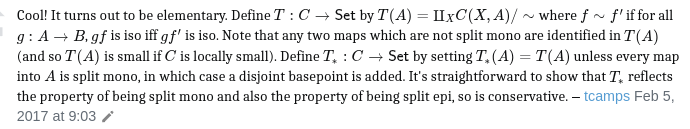
\includegraphics[scale=.5]{freyd.png}
	\end{center}
	\Todo{}
\end{proof}
\begin{definition}[Isomorfismo di categorie]\label{fun_isocat}\index{Categoria!isomorfismo di ---e}\index{Isomorfismo!--- di categorie}\index{Isomorfismo}
	Un isomorfismo di categorie \(\ctC\cong\ctD\) consiste di una coppia di funtori
	\[\xymatrix{
			\ctC \ar[r]^-F & \ctD, & \ctD \ar[r]^-G & \ctC
		}\]
	tali che \(F\cmp G = \Id[\ctD]\) e \(G\cmp F = \Id[\ctC]\).

	Si tratta, evidentemente, di un isomorfismo nella categoria \(\ctCat\) di categorie e funtori di \ref{ex_cat_cat}. In particolare,
	\begin{quote}
		Ogni isomorfismo di categorie induce una biiezione di classi, \(F_0 : \ctC_0\to\ctD_0\), di inversa \(G_0 : \ctD_0\to\ctC_0\), e una biiezione di classi \(F_1 : \ctC_1 \to \ctD_1\), di inversa \(G_1 : \ctD_1\to\ctC_1\) che si decompone in una famiglia `indicizzata' di biiezioni \(F_{XY} : \Hom\ctC(X,Y)\to\Hom\ctD(FX,FY)\), di inversa
		\[\xymatrix{
			\Hom\ctD(FX,FY) \ar[r]^-{G_{FX,FY}} & \Hom\ctC(GFX,GFY) \ar@{=}[r] & \hom(X,Y).
			}\]
	\end{quote}
\end{definition}
\`E più comune trovarsi nella condizione in cui esistono due funtori \(F : \ctC \leftrightarrows \ctD: G\) con la proprietà che esistano \emph{isomorfismi naturali} \(\epsilon : F\cmp G \cong \Id[\ctD]\) ed \(\eta : \Id[\ctC]\cong G\cmp F\). Questa definizione più rilassata di identificazione tra due categorie si dice\emph{equivalenza}, denotata \(\ctC\simeq\ctD\). Vedremo presto che un'equivalenza di categorie \(\ctC\simeq\ctD\) induce biiezioni tra gli hom-insiemi di \(\ctC,\ctD\), ma che le classi degli oggetti di queste possono essere una radicalmente più grande dell'altra (per esempio, \(\ctC_0\) può essere una classe propria, e \(\ctD_0\) un insieme; oppure, esistono categorie dove \(\ctC_0\) ha cardinalità arbitrariamente alta, ma \(\ctD_0\) è un singoletto\dots)
\begin{definition}[Equivalenza di categorie]\label{funtore_equcat}\index{Equivalenza}\index{Categoria!equivalenza di ---e}
	Una \emph{equivalenza di categorie} \(\ctC\simeq\ctD\) consiste di una quadrupla \((F,G,\eta,\epsilon)\), dove
	\begin{itemize}
		\item \(F : \ctC\fun\ctD\) e \(G : \ctD\fun\ctC\) sono funtori in direzioni opposte;
		\item \(\eta : \Id[\ctC] \nat G\cmp F\) e \(\epsilon : F\cmp G \nat \Id[\ctD]\) sono isomorfismi naturali.
	\end{itemize}
	Una equivalenza di categorie si dice \emph{equivalenza aggiunta} se, in più, valgono le seguenti equazioni:
	\begin{itemize}
		\item (equazione zig) la composizione \(\xymatrix{F \ar@{=>}[r]^-{F\whi\eta} & FGF \ar@{=>}[r]^-{\epsilon\whi F} & F}\) è uguale alla trasformazione naturale identica di \(F\);
		\item (equazione zag) la composizione \(\xymatrix{G \ar@{=>}[r]^-{\eta\whi G} & GFG \ar@{=>}[r]^-{G\whi\epsilon} & G}\) è uguale alla trasformazione naturale identica di \(G\).
	\end{itemize}
	Dato \(F\), il funtore \(G\) è detto lo \emph{pseudoinverso} di \(F\), e analogamente \(F\) è lo pseudoinverso del funtore \(G\); i due si caratterizzano a vicenda, ma non in maniera strettamente unica, bensì \emph{a meno di isomorfismo naturale}:
	\begin{quote}
		Se \(\hat G,\tilde G\) sono pseudoinversi dello stesso \(F : \ctC\fun\ctD\), allora esiste un isomorfismo naturale \(\hat G\nat \tilde G\), ottenuto da
		\[\xymatrix{\hat G \ar@{=>}[r]^-{\tilde\eta\whi\hat G } & \hat G F \tilde G \ar@{=>}[r]^-{\tilde G \whi \hat\epsilon} & \tilde G}\]
	\end{quote}
\end{definition}
\begin{hRemark}[A proposito dei nomi `zig' e `zag']{skip}\index{Identità!--- zig e zag}
	Le due equazioni in \ref{funtore_equcat} si rappresentano come incollamenti naturali della forma seguente:
	\[\xymatrix@R=3mm{
		\ctC \ar@{->}[rd]^{F} \ar@/_/@{=}[dd] &  & \ctC \ar@{->}[rd]^{F} \ar@/_/@{=}[dd] &  &  & \ctD \ar@{->}[rd]^{G} \ar@/_/@{=}[dd]\ddtwocell<\omit>{<-2>\epsilon} &  & \ctD \ar@{->}[rd]^{G} \ar@/_/@{=}[dd] &  \\
		& \ctD \ar@{}[dr]|=\ar@{->}[ld]|-{G} \ar@/^/@{=}[dd] &  & \ctD \ar@/^/@{=}[dd] &  &  & \ctC \ar@{}[dr]|=\ar@{->}[ld]|-{F}\ddtwocell<\omit>{<2>\eta} \ar@/^/@{=}[dd] &  & \ctC\dltwocell<\omit>{\Id[G]\kern.75em} \ar@/^/@{=}[dd] \\
		\ctC\uutwocell<\omit>{<2>\eta} \ar@{->}[rd]_{F} &  & \ctC \urtwocell<\omit>{\kern.75em\Id[F]}\ar@{->}[rd]_{F} &  &  & \ctD \ar@{->}[rd]_{G} &  & \ctD \ar@{->}[rd]_{G} &  \\
		& \ctD\uutwocell<\omit>{<-2>\epsilon} &  & \ctD &  &  & \ctC &  & \ctC
		}\]
	A causa della forma di questi diagrammi (due triangoli sono incollati insieme ed \(F,G\) formano uno zig-zag di frecce in direzioni opposte), esse sono colloquialmente chiamate \emph{identità zig-zag} o identità triangolari (o identità \emph{di aggiunzione}, si vedrà nel \autoref{cap_aggiunti}).
\end{hRemark}
Sorprendentemente, la nozione di equivalenza di categorie non è più debole della nozione di equivalenza aggiunta, ossia, è sempre possibile indurre un'equivalenza aggiunta a partire da una equivalenza.
\begin{lemma}\label{eq_sono_eqadj}\index{Equivalenza aggiunta}
	Ogni equivalenza di categorie \((F,G,\eta,\xi)\) induce una equivalenza aggiunta \((F,G,\eta,\epsilon)\), dove \(\eta,\epsilon\) soddisfano le identità zig-zag.
\end{lemma}
\begin{proof}
	Data un'equivalenza di categorie \(\ctC\simeq\ctD : (F,G,\eta,\epsilon)\) come in \ref{funtore_equcat}, definiamo a partire da \(\xi : FG\nat \Id[\ctD]\) una trasformazione naturale
	\[\xymatrix@C=2cm{
		\epsilon : FG \ar@{=>}[r]^-{FG\whi \xi^{-1}} & FGFG \ar@{=>}[r]^-{F\whi\eta^{-1}\whi G} & FG \ar@{=>}[r]^-\xi & \Id[\ctD]
		}\]
	per composizione verticale. Dobbiamo ora dimostrare che \(\eta,\epsilon\) soddisfano le due identità zig e zag. Per farlo, ragioniamo equazionalmente e troviamo che la naturalità di \(\eta\) in \(\xi\) implica che
	\begin{align*}
		(G\whi\epsilon)\cmp(\eta \whi G) & = (G\whi\xi )\cmp(GF\whi\eta^{-1}\whi G)\cmp\underline{(GFG\whi\xi^{-1})\cmp(\eta\whi G)}      \\
		                                 & = (G\whi\xi )\cmp(GF\whi\eta^{-1}\whi G)\cmp(\eta\whi GFG)\cmp(G\whi \xi^{-1})                 \\
		                                 & = (G\whi\xi )\cmp\underline{(\eta\whi G)\cmp(\eta^{-1}\whi G)}\cmp(G\whi \xi^{-1})             \\
		                                 & = \underline{(G\whi\xi )\cmp(G\whi \xi^{-1})}                                                  \\
		                                 & =\Id[G].                                                                                       \\
		(\epsilon\whi F)\cmp(F\whi\eta)  & = (\xi\whi F)\cmp\underline{(F\whi\eta^{-1}\whi GF)\cmp(FG\whi \xi^{-1}\whi F)}\cmp(F\whi\eta) \\
		                                 & = \underline{(\xi\whi F)\cmp(\xi^{-1}\whi F)}\cmp(F\whi\eta^{-1})\cmp(F\whi\eta)               \\
		                                 & = \underline{(F\whi\eta^{-1})\cmp(F\whi\eta)}                                                  \\
		                                 & = \Id[F].
	\end{align*}
	Questo conclude la dimostrazione. (In ciascuna riga, operiamo con una riscrittura sulla parte sottolineata)
\end{proof}
\begin{definition}\label{funtore_wequcat}\index{Equivalenza debole}
	Una equivalenza debole di categorie è un funtore \(F : \ctC \fun\ctD\) che sia pieno, fedele ed essenzialmente suriettivo.
\end{definition}
\begin{remark}\label{eq_implies_weq_AC_eq}\index{Assioma della scelta}\index{Equivalenza}
	Ogni equivalenza di categorie è un'equivalenza debole di categorie. Il viceversa, che consiste nel costruire uno pseudoinverso per un funtore \(F : \ctC\fun\ctD\) che sia un'equivalenza debole, è dimostrabile assumendo un assioma della scelta (per classi: ogni funzione di classe \(K : \ctC_0 \to \ctD_0\) suriettiva ammette una sezione, ossia se ogni \(K^{-1}D\) è non vuota, è possibile definire una funzione di classe \(H : D\mapsto HD \in K^{-1}D\)).
	\begin{itemize}
		\item Se \(F\) è un'equivalenza di categorie, per \ref{eq_sono_eqadj} possiamo metterci nella situazione in cui \(F\) è un'equivalenza aggiunta con pseudoinverso \(G : \ctD\fun\ctC\). Allora per ogni \(f : X\to Y\) in \(\ctC\) abbiamo un quadrato commutativo
		      \[\xymatrix{
			      X\ar[r]^-{\eta_X}\ar[d]_f & GFX \ar[d]\ar[d]^{GFf}\\
			      Y \ar[r]_-{\eta_Y} & GFY
			      }\]
		      per la naturalità di \(\eta\); allora se \(Ff_1 = Ff_2\), anche \(GFf_1 = GFf_2\), cioè
		      \[\eta_Y\cmp f_1 \cmp \eta_X^{-1} = GFf_1 = GFf_2 = \eta_Y\cmp f_2 \cmp \eta_X^{-1}\]
		      Quindi, siccome tutti gli isomorfismi sono mono ed epi, ovvero cancellabili sia destra che a sinistra, \(f_1 = f_2\). Questo mostra che \(F\) è fedele. Data ora una freccia \(g : FA\to FB\) in \(\ctD\), la freccia \(Gg : GFA\to GFB\) è un morfismo di \(\ctC\), e possiamo considerare il diagramma
		      \[\xymatrix{
			      FA \ar@{=}[dr]\ar[r]^-{\eta_{FA}}& FGFA \ar[d]_{\epsilon_A}\ar[r]^-{FGg} & FGFB \ar[d]^{\epsilon_B}\ar[r]^-{\eta_{FB}^{-1}}& FB \\
			      & FA \ar[r]_-g& FB \ar@{=}[ur]&
			      }\]
		      (per la naturalità di \(\epsilon\) e per l'equazione zig); Quindi \(F\big(\eta_B^{-1}\cmp Gg\cmp \eta_A\big) = g\); questo mostra che \(F\) è pieno.

		      Ogni oggetto \(X\in\ctD_0\) poi è della forma \(F(GX) \cong X\) mediante l'isomorfismo (naturale in \(X\)!) dato da \(\epsilon\).
		\item Nell'altro verso abbiamo bisogno di una forma di assioma della scelta: siccome \(F\) è essenzialmente suriettivo, possiamo scegliere un \(C\in F_0^{-1}D\) per ogni \(D\) (e degli isomorfismi \(\epsilon : FGC \cong C\)); questo definisce una funzione di classe \(G_0 : \ctD_0\to\ctC_0\) che è la corrispondenza sugli oggetti del funtore \(G : \ctD\fun\ctC\) che stiamo costruendo. Gli isomorfismi \(\epsilon : FGC \to C\) sono le componenti di una trasformazione naturale se definiamo \(G\) sulle frecce come segue: dato \(h : C\to C'\), il quadrato
		      \[\xymatrix{
				      FGC \ar[r]\ar[d]& C \ar[d]^h\\
				      FGC' \ar[r]& C'
			      }\]
		      commuta quando la freccia verticale a sinistra sia \(\epsilon_{C'}^{-1}\cmp h\cmp \epsilon_C : FG\), e siccome \(F\) è pienamente fedele esiste un'unica freccia \(a : GC \to GC'\) tale che \(Fa = \epsilon_{C'}^{-1}\cmp h\cmp \epsilon_C\); chiamando \(Gh=a\), questo significa che \(\epsilon_{C'}\cmp FGh = h\cmp \epsilon_C\), che è la naturalità di \(\epsilon\) in \(h\).

		      Per determinare \(\eta : \Id[\ctC] \nat GF\), consideriamo \(\epsilon_{FC} : FGFC \to FC\): siccome \(F\) è pienamente fedele, esiste un'unica freccia \(\eta^{-1}_C : GFC\to C\) tale che \(F(\eta^{-1}_C) = \epsilon_{FC}\), e (dato che un funtore pienamente fedele riflette gli isomorfismi, \ref{prop_preserva_riflette}) \(F(\eta^{-1}_C)=F(\eta_C)^{-1}_C\) per un'unica freccia \(\eta_C : C\to GFC\). Un ragionamento simile a prima ne mostra la naturalità.
	\end{itemize}
\end{remark}
Gli isomorfismi di categorie sono relativamente rari, poiché le proprietà di molte categorie sono invarianti per una nozione molto più debole di identificazione.
Gli esempi di categorie equivalenti ma non isomorfe sono molto comuni. Ad esempio, ogni gruppoide è equivalente a una unione disgiunta di gruppi (guardati come gruppoidi con un solo oggetto), senza che questa equivalenza sia un isomorfismo; e il gruppoide fondamentale \(\Pi_1(X)\) di uno spazio topologico \(X\) connesso per archi è una categoria equivalente, ma non isomorfa, a \(\pi_1(X,x_0)\) per una opportuna scelta di un punto di base \(x_0\in X\). Questo suggerisce che due categorie piccole con due insiemi degli oggetti di diversa cardinalità possono essere equivalenti; un esempio estremo è questo: se \(A\) è un insieme e \(A^\chi\) il gruppoide caotico di \ref{ex_cat_codiscreta}, esiste un unico funtore \(F : A^\chi \to \ctTerm\), definito nell'unico modo possibile, ed esso è un'equivalenza (debole). In particolare (invitiamo chi legge a completare i dettagli per esercizio)
\begin{remark}\index{Categoria!--- isomorfismo generico}
	La categoria `isomorfismo generico' di \ref{ex_cat_iso},
	\[\xymatrix@C=7ex{0 \ar@<.7ex>[r]^u \ar@(dl,ul)[] & 1 \ar@<.7ex>[l]^{u^{-1}} \ar@(ur,dr)[]}\]
	è equivalente alla categoria \(\ctTerm\).
\end{remark}
\begin{example}\index{Categoria!equivalenza di ---e}\index{Equivalenza!--- di categorie}
	\Todo{La categoria delle matrici di \ref{ex_cat_matrici} è equivalente, senza essere isomorfa, a \(\ctVect\).}
\end{example}
L'esercizio \ref{ex_monepi_2} chiederà di dimostrare che le due non possono essere isomorfe.

Finiamo la sezione caratterizzando i monomorfismi in \(\ctCat\): si tratta di funtori \(F : \ctC \fun\ctD\) con la proprietà che sia \(F_0 : \ctC_0\to\ctD_0\) che ogni \(F_{XY} : \Hom\ctC(X,Y) \to \Hom\ctD(F_0X,F_0Y)\) sono funzioni iniettive.
\begin{proposition}\label{mona_in_cat}\index{Monomorfismo!--- in \(\ctCat\)}
	La classe dei monomorfismi di \(\ctCat\) consiste dei funtori \(F : \ctC\fun\ctD\) che sono fedeli e iniettivi sugli oggetti (cioè \(F_0\) e tutte le \(F_{XY}\) in \ref{def_alternativa_funtore} sono entrambe funzioni iniettive).
\end{proposition}
\begin{proof}
	Se sono dati due funtori \(H,K:\ctJ \fun \ctC\), tali che \(F\cmp H = F\cmp K\), ed \(F\) è iniettivo sugli oggetti, allora per ogni \(J\in\ctJ_0\) si ha \(HJ=KJ\); similmente, se \(F\) è iniettivo sui morfismi, si ha \(Hf = Gf\) per ogni \(f : X\to Y\) in \(\ctC\).

	Se \(F : \ctC \fun\ctD\) è un mono in \(\ctCat\), quando \(X,Y \in\ctC_0\) si rappresentano come funtori \(X,Y : \ctTerm \fun \ctC\) al modo di \ref{tante_cose_sono_diag}, è evidente che \(F\cmp X\) è l'oggetto \(F_0X\) (risp., \(F\cmp Y\) è \(F_0 Y\)): se questi ultimi sono uguali, allora \(X=Y\). In maniera simile, è possibile mostrare che ogni \(F_{XY}\) è iniettiva, presentando \(f,g : X\to Y\) come funtori \(\genArrow \fun \ctC\).

	Questo conclude la dimostrazione.
\end{proof}
\begin{definition}[Funtori iniziali e finali]\label{def_fun_initfin}\index{Funtore!--- iniziale}\index{Funtore!--- finale|see {Funtore iniziale}}
	Un funtore \(F : \ctC\fun\ctD\) si dice \emph{iniziale} se per ogni oggetto \(D\in\ctD\) la categoria comma \((D/F)\) i cui oggetti sono coppie \((X,f : D\to FX)\) è non vuota e connessa (nel senso che \(\pi_0^\ctCat(D/F)\), si veda \ref{exe_cpt_conn}, \ref{ex_fun_cpt_conn}, ha un unico elemento).

	In altre parole, \(F : \ctC\fun\ctD\) si dice iniziale se le due condizioni seguenti sono soddisfatte:
	\begin{enumtag}{fi}
		\item \label{fi_1} per ogni \(D\in\ctD\), l'insieme \(\sum_X\Hom\ctD(D,FX)\) è non vuoto;
		\item \label{fi_2} date due frecce \(D\to FX, D\to FY\) in \(\ctD\), esiste una successione finita di oggetti \(\tup An,\) e morfismi \(A_i \leftrightarrows A_{i+1}\) (in una delle due direzioni) tali che ogni triangolo nel diagramma
		% https://q.uiver.app/#q=WzAsNyxbMCwxLCJGWCJdLFsxLDEsIkZBXzAiXSxbMiwxLCJGQV8xIl0sWzMsMSwiXFxkb3RzIl0sWzQsMSwiRkFfbiJdLFs1LDEsIkZZIl0sWzIsMCwiRCJdLFs2LDBdLFs2LDFdLFs2LDJdLFs2LDRdLFs2LDVdLFswLDEsIiIsMCx7InN0eWxlIjp7ImhlYWQiOnsibmFtZSI6Im5vbmUifX19XSxbMSwyLCIiLDAseyJzdHlsZSI6eyJoZWFkIjp7Im5hbWUiOiJub25lIn19fV0sWzIsMywiIiwwLHsic3R5bGUiOnsiaGVhZCI6eyJuYW1lIjoibm9uZSJ9fX1dLFszLDQsIiIsMCx7InN0eWxlIjp7ImhlYWQiOnsibmFtZSI6Im5vbmUifX19XSxbNCw1LCIiLDAseyJzdHlsZSI6eyJoZWFkIjp7Im5hbWUiOiJub25lIn19fV1d
		\[\begin{tikzcd}
				&& D \\
				FX & {FA_0} & {FA_1} & \dots & {FA_n} & FY
				\arrow[from=1-3, to=2-1]
				\arrow[from=1-3, to=2-2]
				\arrow[from=1-3, to=2-3]
				\arrow[from=1-3, to=2-5]
				\arrow[from=1-3, to=2-6]
				\arrow[no head, from=2-1, to=2-2]
				\arrow[no head, from=2-2, to=2-3]
				\arrow[no head, from=2-3, to=2-4]
				\arrow[no head, from=2-4, to=2-5]
				\arrow[no head, from=2-5, to=2-6]
			\end{tikzcd}\]
		sia commutativo.
	\end{enumtag}
	Diciamo che \(F : \ctC\fun\ctD\) è \emph{finale} se il funtore opposto \(F^\op : \ctC^\op\fun\ctD^\op\) (come in \ref{es_di_funtori}) è iniziale.
\end{definition}
\begin{remark}[Condizione di Ore]\label{condizione_ore}\index{Funtore!condizione di Ore per un ---}\index{Funtore!--- iniziale}
	Una condizione più forte dell'inizialità, molto comune e più facile da verificare, è la \emph{condizione di Ore}: \(F : \ctC\fun\ctD\) la soddisfa se
	\begin{itemize}
		\item per ogni \(D\in\ctD\), l'insieme \(\sum_X\Hom\ctD(D,FX)\) è non vuoto;
		\item per ogni \(D\) e ogni \(u : D\to FX\), \(v : D\to FY\) esiste un modo di `completare il quadrato'
		      \[\xymatrix{
				      D\ar[r]^u\ar[d]_v & FX \ar@{.>}[d]^{Ff}\\
				      FY \ar@{.>}[r]_{Fg} & FZ
			      }\]
		      con due frecce \(X \xto fZ \xot g Y\) di \(\ctC\).
	\end{itemize}
\end{remark}
Si osservi che la composizione \(G\cmp F\) di funtori dove \(G\) soddisfa la condizione di Ore ed \(F\) è tale che ogni categoria \((Z/F)\) è non vuota, soddisfa a sua volta la condizione di Ore:
\begin{itemize}
	\item nella categoria comma \((D/GF)\) esiste almeno una freccia \(D \xto u GX \xto{Gv} GFY\);
	\item Se viene dato un diagramma \(\xymatrix{GFX & \ar[l]_-u D\ar[r]^-v & GFY}\) (dove non necessariamente \(u,v\) sono della forma \(D\to G\bullet\xto{G\bullet}GFX\) e \(D\to G\bullet\xto{G\bullet}GFY\)), esso si può completare come
	      \[\xymatrix{
		      D \ar[r]^u\ar[d]_v& GFX\ar@{.>}[d]\ar@{.>}@/^1pc/[ddr]\\
		      GFY \ar@{.>}[r]\ar@{.>}@/_1pc/[drr] & GZ\ar@{.>}[dr]_{\exists w} \\
		      && GFV
		      }\]
\end{itemize}
\begin{theorem}
	Il \emph{prodotto} di due funtori \(F : \ctI\fun\ctC\) e	\(G : \ctJ\fun\ctD\) è il funtore
	\[\xymatrix@R=0cm{
		\ctI\times\ctJ \ar[r] & \ctC\times\ctD \\
		(I,J) \ar@{|->}[r] & (FI,GJ)
		}\]
	(notazione come in \ref{}).

	Nelle stesse notazioni, se \(F,G\) sono funtori iniziali come in \ref{}, allora \(F\times G\) è iniziale.
\end{theorem}
\begin{proof}
	\Todo{Prodotto di iniziali è iniziale}
	Va dimostrato che per ogni oggetto \((C,D)\) la categoria comma \(((C,D)/F\times G)\) è non vuota e connessa. Evidentemente è non vuota dato che dei morfismi \(C\to FX\) e \(D\to GY\) esistono separatamente in \((C/F)\) e \((D/G)\). Va mostrato, poi, che ogni coppia di oggetti in \(((C,D)/F\times G)\) è connessa da uno zigzag di morfismi. Per fare questo, va risolto il seguente problema: esistono certamente delle successioni finite
	\[\xymatrix@C=8mm{
		&&C\ar[dr]\ar[dl]\ar[dll]\ar[drr] &&&&& D\ar[dr]\ar[dl]\ar[dll]\ar[drr]\\
		FI\ar@{-}[r] & FX_1\ar@{-}[r] & \dots\ar@{-}[r] & FX_\ell\ar@{-}[r] & FI' & GJ\ar@{-}[r] & GY_1\ar@{-}[r] & \dots\ar@{-}[r] & GY_m\ar@{-}[r] & GJ'
		}
	\]
	di triangoli commutativi in \(\ctC\) e \(\ctD\) separatamente, e però non si può garantire che esse siano della stessa lunghezza (come è invece richiesto per assemblare uno zig-zag di morfismi in \(((C,D)/F\times G)\)). Non è difficile risolvere il problema, `degenerando' alcuni pezzi delle successioni per adattarne la lunghezza; se ad esempio \(\ell=2,m=1\) le successioni sopra sono della forma
	\[\xymatrix{
		&C\ar[dr]|{x_2}\ar[dl]_{c}\ar[d]|{x_1}\ar[drr]^{c'} &&&& D\ar[d]|{y_1}\ar[dr]^{d'}\ar[dl]_d \\
		FI\ar@{->}[r]_{u_0} & FX_1\ar@{<-}[r]_{u_1} & FX_2\ar@{->}[r]_{u_2} & FI' &
		GJ\ar@{<-}[r]_{v_0} & GY_1 \ar@{->}[r]_{v_1} & GJ'
		}\]
	è semplice generare la successione seguente dove indichiamo i morfismi di \(\ctC\times\ctD\) come doppie frecce per chiarezza:
	\[\xymatrix@C=1.2cm@R=1.5cm{
		&(C,D)\ar@/_.5pc/@<.25em>[dl]\ar@/_.5pc/@<-.25em>[dl]_{(c,d)}\ar@<-.25em>[d]|\hole\ar@<.25em>[d]|{(x_1,d)}\ar@<-.25em>[dr]_{(x_2,y_1)}\ar@<.25em>[dr]\ar[drr]\ar@<.5em>[drr]^{(c',d')}\\
		(FI,GJ)\ar@<.225em>[r]\ar@<-.225em>@{=}[r]_{(u_0,\id)} & (FX_1,GJ) & (FX_2,GY_1)\ar@<.225em>[l]^{(u_1,v_0)}\ar@<-.225em>[l] \ar@<.225em>[r]\ar@<-.225em>[r]_{(u_2,v_1)} & (FI',GJ').
		}
	\]
	Si noti in particolare che se \(\ell,m\) sono le rispettive lunghezze delle successioni trovare in \(\ctC,\ctD\) separatamente, la stima \(k\le \ell+m\) della lunghezza \(k\)	della successione di triangoli in \(((C,D)/F\times G)\) è solo un limite superiore. Si provi, per esercizio, a formalizzare il caso generale con una ricetta `induttiva' per lunghezze e orientazioni generiche (concordanti, e discordanti\dots).
\end{proof}
\begin{hTheorem}[Inizialità degli ordinali tra i diagrammi filtrati]{skip}\index{Funtore!--- iniziale}
	Per ogni categoria \(\ctJ\) (piccola e) filtrata nel senso di \ref{def_cat_filtrata}, esiste un funtore iniziale \(K : P_\ctJ\fun\ctJ\), di dominio un preordine (si veda \ref{ex_cat_ordini}) diretto (si veda \ref{contro_esempi_filt}).
\end{hTheorem}
\begin{proof}
	Grazie a \ref{estensione_filtrata}, sappiamo che ogni sottocategoria finita \(\ctF\subseteq\ctJ\) ammette una estensione a un funtore \(\ctF^\rhd\fun\ctJ\); in particolare (si veda \ref{def_cono_su_C}) il vertice del cocono così ottenuto è terminale in \(\ctF\). Ora, il poset \(P_\ctJ = (\{\ctF_\alpha\},\subseteq)\) delle sottocategorie finite \(\ctF\) di \(\ctJ\) (in ciascuna delle quali c'è un oggetto terminale \(\infty_\alpha\)) è diretto (è sufficiente considerare l'unione di due sottocategorie finite), e possiamo definire un funtore
	\[\dmFun{K}{P_\ctJ}{\ctJ}\]
	ottenuto mandando \(\ctF_\alpha\) nell'oggetto terminale \(\infty_\alpha\) di \(J_\alpha^*\), e una inclusione \(\ctF_\alpha\subseteq\ctF_\beta\) nell'ovvia freccia \(\infty_\alpha\to\infty_\beta\).

	Questo funtore è iniziale: per ogni oggetto \(J\in\ctJ_0\), \(K\{J\}=J\), e quindi esiste \(\Id[J] : J\to K\{J\}\). Se poi \(f : J\to K\ctF_\alpha\) e \(g : J\to K\ctF_\beta\), allora definiamo \(\ctF_\gamma := \ctF_\alpha\cup\ctF_\beta\cup\{f,g\}\); evidentemente, le inclusioni \(\ctF_\alpha,\ctF_\beta\subseteq\ctF_\gamma\) realizzano la seconda condizione di Ore \ref{condizione_ore}.
\end{proof}
\begin{theorem}
	Una categoria \(\ctJ\) è setacciata nel senso di \ref{def_cat_setacciata} se e solo se il funtore diagonale di \ref{es_di_funtori}.\ref{exfun_3}
	\[\dmFun{\Delta}{\ctJ}{\ctJ\times\ctJ}\]
	è iniziale nel senso di \ref{def_fun_initfin}.
\end{theorem}
\begin{proof}
	\Todo{setacciata iff diagonale iniziale}
\end{proof}
\begin{theorem}
	Se \(\ctI,\ctJ\) sono due categorie setacciate, il prodotto \(\ctI\times\ctJ\) è una categoria setacciata.
\end{theorem}
\begin{proof}
	\`E un corollario immediato del fatto che il prodotto di funtori iniziali è iniziale, si veda \ref{}, insieme al fatto che il funtore prodotto \(\Delta_{\ctI\times\ctJ}\) risulta dalla composizione
	\[\xymatrix{
			\ctI\times\ctJ \ar[r]^{\Delta_\ctI\times\Delta_\ctJ} & \ctI\times\ctI\times \ctJ\times\ctJ\ar@{=}[r]^\sim & \ctI\times\ctJ\times \ctI\times\ctJ
		}\]
\end{proof}
Grazie a \ref{} otteniamo una dimostrazione alternativa del fatto che ogni categoria filtrata $\ctJ$ è setacciata, perché possiamo mostrare (cosa che in \ref{} non potevamo usare, dato che ci mancava la nozione di funtore	iniziale) che se $\ctJ$ è una categoria filtrata, $\Delta_\ctJ$ è iniziale. 
\begin{proof}
	Se $\ctJ$ è filtrata, dobbiamo mostrare che per ogni oggetto $(J,J')$ di $\ctJ_0\times\ctJ_0$, la categoria	comma \((J,J')/\Delta_\ctJ\) è non vuota e connessa. Del resto, il fatto che esista almeno una freccia $(u,v) : (J,J') \to (J^*,J^*)$ è esattamente la proprietà \ref{cf_1} di \ref{def_cat_filtrata}; la proprietà \ref{cf_2} consiste nel dimostrare che ogni coppia di oggetti 
	\[\xymatrix{
		(X,Y) & (J,J')& (A,B)
	}\]
	di \((J,J')/\Delta_\ctJ\) è connessa da uno zig zag di triangoli commutativi; chiaramente, per definizione di cosa sia la categoria prodotto $\ctJ\times\ctJ$...	% Per ogni oggetto \(J\in\ctJ_0\), esiste un oggetto \(\infty_J\) di \(\ctJ\) che è terminale in \(\ctJ\), e quindi per ogni coppia di oggetti \((J,J')\) esiste un morfismo \(\infty_J\to J\) e uno \(\infty_{J'}\to J'\); questi due morfismi sono sufficienti a mostrare che la categoria comma è connessa, e non vuota perché contiene almeno l'oggetto \((\infty_J,\infty_{J'})\).
\end{proof}
\begin{figure}
	\begin{center}
		\begin{tikzpicture}[
				x=4em, y=4em,
				dot/.style={
						circle,
						fill=#1,
						inner sep=0pt,
						outer sep=2pt,
						minimum size=4pt,
						draw=none,
					},
				wrap/.style={
						fill=black!5,
						draw=gray,
						rounded corners,
						inner sep=.5em,
					},
			]

			\def\seedX{4}
			\def\sizeX{5}
			\pgfmathsetseed{\seedX}
			\GimmeBounds{\seedX}{\sizeX}

			\begin{scope}[local bounding box=UP]
				\pgfmathsetseed{\seedX}
				\foreach \i in {1,...,3} {
						\pgfmathsetmacro{\x}{(rnd-\xmid)/ifthenelse(\xmax==\xmin,1,\xmax-\xmin)}
						\pgfmathsetmacro{\y}{(rnd-\ymid)/ifthenelse(\ymax==\ymin,1,\ymax-\ymin)}
						\path node[dot=black] (J\i) at (\x,\y) {};
					}
				\foreach \i in {4,...,5} {
						\pgfmathsetmacro{\x}{(rnd-\xmid)/ifthenelse(\xmax==\xmin,1,\xmax-\xmin)}
						\pgfmathsetmacro{\y}{(rnd-\ymid)/ifthenelse(\ymax==\ymin,1,\ymax-\ymin)}
						\path node[dot=black!5] (J\i) at (\x,\y) {};
					}

				\path node[dot=ibmOrange] (Jinfty) at (-0.3,-0.3) {};
			\end{scope}

			\begin{scope}[yshift=-6em, local bounding box=DN]
				\pgfmathsetseed{\seedX}
				\foreach \i in {1,...,3} {
						\pgfmathsetmacro{\x}{(rnd-\xmid)/ifthenelse(\xmax==\xmin,1,\xmax-\xmin)}
						\pgfmathsetmacro{\y}{(rnd-\ymid)/ifthenelse(\ymax==\ymin,1,\ymax-\ymin)}
						\path node[dot=black] (J\i') at (\x,\y) {};
					}
				\foreach \i in {4,...,5} {
						\pgfmathsetmacro{\x}{(rnd-\xmid)/ifthenelse(\xmax==\xmin,1,\xmax-\xmin)}
						\pgfmathsetmacro{\y}{(rnd-\ymid)/ifthenelse(\ymax==\ymin,1,\ymax-\ymin)}
						\path node[dot=gray] (J\i') at (\x,\y) {};
					}

				\path node[dot=ibmBlue] (Jinfty') at (0.1,0.1) {};
			\end{scope}

			\foreach \i in {1,...,3} \draw[-latex, gray] (J\i) -- (Jinfty);
			\foreach \i in {1,...,5} \draw[-latex, gray] (J\i') -- (Jinfty');
			\draw[-latex] (Jinfty) -- (Jinfty');

			\begin{scope}[xshift=4cm, local bounding box=JJ]
				\pgfmathsetseed{\seedX}
				\foreach \i in {1,...,10} {
						\pgfmathsetmacro{\x}{(rnd-\xmid)/ifthenelse(\xmax==\xmin,1,\xmax-\xmin)}
						\pgfmathsetmacro{\y}{(rnd-\ymid)/ifthenelse(\ymax==\ymin,1,\ymax-\ymin)}
						\path node[dot=gray] (J\i') at (\x,\y) {};
					}
			\end{scope}

			\begin{scope}[on background layer]
				\path node[wrap, fit=(UP)] (D) {};
				\path node[wrap, fit=(DN)] (C) {};
				\path node[wrap, fit=(JJ)] (ctJ) {};
				\node[left=.25em of D] {$\ctI'$};
				\node[left=.25em of C] {$\ctI''$};
				\node[right=.25em of ctJ] {$\ctJ$};
			\end{scope}
		\end{tikzpicture}
		\caption{Costruzione di un funtore iniziale verso una categoria filtrata \(\ctJ\); \(\orangeDot\) è il vertice di un cocono nella categoria \(\ctI'\), \(\blueDot\) nella categoria \(\ctI''\supseteq\ctI'\), e questa proprietà determina un'unica freccia \(\orangeDot\to\blueDot\).}
		\label{fig_TODO}
	\end{center}
\end{figure}
\begin{esercizi}
	\item \label{ex_monepi_1} In \ref{mona_in_cat} abbiamo dimostrato che i monomorfismi in \(\ctCat\) sono i funtori iniettivi \emph{sugli oggetti e sui morfismi}. Trovare un funtore che non è iniettivo sugli oggetti, ma lo è sui morfismi, e mostrare che non è un mono. Si faccia lo stesso per un funtore che non è iniettivo sui morfismi, ma lo è sugli oggetti.
	\item \label{ex_monepi_2} Fissato un campo \(\bbF\), mostrare che \(\ctMat\) e \(\ctVect\) \emph{non possono essere} categorie isomorfe (suggerimento: si veda la definizione di \emph{anima} di una categoria in \ref{def_cuore}: \(\ctC^\text{an} := \sum_{C\in\ctC_0} \ctC_\cong(C,C)\); mostrare che due categorie isomorfe hanno anime isomorfe; mostrare che l'anima di \(\ctMat\) e quella di \(\ctVect\) non sono isomorfe.)
	\item \label{ex_monepi_3} Costruire un'equivalenza di categorie tra la categoria dei sistemi dinamici discreti di \ref{ex_cat_dyn} e la categoria delle rappresentazioni, \ref{es_fun_repre}, del monoide \((\bbN,+,0)\); è un isomorfismo? Mostrare che \(\bbN\) è in maniera naturale un oggetto \(\bsN=(* \xto 0 \bbN \xto{\blank+1} \bbN)\) di \(\ctDyn\), che soddisfa la proprietà (\emph{universale}) seguente:
	\begin{quote}
		Per ogni oggetto \(\bsX=(X,x_0,f)\) di \(\ctDyn\) esiste uno e un solo morfismo nell'insieme \(\Hom\ctDyn(\bsN,\bsX)\).
	\end{quote}
	\item \label{ex_monepi_4} Se \(\ctC\) è una categoria, un \emph{generatore} è un oggetto \(G\) con la proprietà che
	\begin{quote}
		bla
	\end{quote}
	Mostrare che \(G\) è un generatore di \(\ctC\) se e solo se il funtore \(\Hom\ctC(G,-)\) è fedele.
	\item \label{ex_monepi_5} Guardando un monoide come una categoria con un solo oggetto, al modo di \ref{mon_sonocat}, mostrare che
	\begin{itemize}
		\item se \(M,N\) sono gruppi, \(\susp f : \susp N\to \susp M\) è un funtore iniziale se e solo se \(f\) è un omomorfismo suriettivo;
		\item se \(M,N\) sono monoidi, ed \(f : N\to M\) è un omomorfismo suriettivo, allora \(\susp f : \susp N\to \susp M\) è un funtore iniziale, ma non è vero il viceversa (esiste un omomorfismo non suriettivo, che induce un funtore iniziale). % l'inclusione di N in Z.
	\end{itemize}
	L'omomorfismo \(T(\bbR,2) \to M(\bbR,2)\) (rispetto alla moltiplicazione) che include le matrici \(2\times 2\) triangolari superiori \(\left(\begin{smallmatrix} a	&	b\\ 0 & c		\end{smallmatrix}\right)\)	nelle matrici \(2\times 2\) induce un funtore iniziale?
	% \`E possibile trovare un criterio generale così che un omomorfismo di monoidi \(f : N\to M\) induca un funtore \(\susp f : \susp N\to \susp M\) iniziale?
\end{esercizi}